\documentclass{article}

\usepackage[T1]{fontenc}
\usepackage{iclr2027_conference,times}
%%%%% NEW MATH DEFINITIONS %%%%%

\usepackage{amsmath,amsfonts,bm}

% Mark sections of captions for referring to divisions of figures
\newcommand{\figleft}{{\em (Left)}}
\newcommand{\figcenter}{{\em (Center)}}
\newcommand{\figright}{{\em (Right)}}
\newcommand{\figtop}{{\em (Top)}}
\newcommand{\figbottom}{{\em (Bottom)}}
\newcommand{\captiona}{{\em (a)}}
\newcommand{\captionb}{{\em (b)}}
\newcommand{\captionc}{{\em (c)}}
\newcommand{\captiond}{{\em (d)}}

% Highlight a newly defined term
\newcommand{\newterm}[1]{{\bf #1}}


% Figure reference, lower-case.
\def\figref#1{figure~\ref{#1}}
% Figure reference, capital. For start of sentence
\def\Figref#1{Figure~\ref{#1}}
\def\twofigref#1#2{figures \ref{#1} and \ref{#2}}
\def\quadfigref#1#2#3#4{figures \ref{#1}, \ref{#2}, \ref{#3} and \ref{#4}}
% Section reference, lower-case.
\def\secref#1{section~\ref{#1}}
% Section reference, capital.
\def\Secref#1{Section~\ref{#1}}
% Reference to two sections.
\def\twosecrefs#1#2{sections \ref{#1} and \ref{#2}}
% Reference to three sections.
\def\secrefs#1#2#3{sections \ref{#1}, \ref{#2} and \ref{#3}}
% Reference to an equation, lower-case.
\def\eqref#1{equation~\ref{#1}}
% Reference to an equation, upper case
\def\Eqref#1{Equation~\ref{#1}}
% A raw reference to an equation---avoid using if possible
\def\plaineqref#1{\ref{#1}}
% Reference to a chapter, lower-case.
\def\chapref#1{chapter~\ref{#1}}
% Reference to an equation, upper case.
\def\Chapref#1{Chapter~\ref{#1}}
% Reference to a range of chapters
\def\rangechapref#1#2{chapters\ref{#1}--\ref{#2}}
% Reference to an algorithm, lower-case.
\def\algref#1{algorithm~\ref{#1}}
% Reference to an algorithm, upper case.
\def\Algref#1{Algorithm~\ref{#1}}
\def\twoalgref#1#2{algorithms \ref{#1} and \ref{#2}}
\def\Twoalgref#1#2{Algorithms \ref{#1} and \ref{#2}}
% Reference to a part, lower case
\def\partref#1{part~\ref{#1}}
% Reference to a part, upper case
\def\Partref#1{Part~\ref{#1}}
\def\twopartref#1#2{parts \ref{#1} and \ref{#2}}

\def\ceil#1{\lceil #1 \rceil}
\def\floor#1{\lfloor #1 \rfloor}
\def\1{\bm{1}}
\newcommand{\train}{\mathcal{D}}
\newcommand{\valid}{\mathcal{D_{\mathrm{valid}}}}
\newcommand{\test}{\mathcal{D_{\mathrm{test}}}}

\def\eps{{\epsilon}}


% Random variables
\def\reta{{\textnormal{$\eta$}}}
\def\ra{{\textnormal{a}}}
\def\rb{{\textnormal{b}}}
\def\rc{{\textnormal{c}}}
\def\rd{{\textnormal{d}}}
\def\re{{\textnormal{e}}}
\def\rf{{\textnormal{f}}}
\def\rg{{\textnormal{g}}}
\def\rh{{\textnormal{h}}}
\def\ri{{\textnormal{i}}}
\def\rj{{\textnormal{j}}}
\def\rk{{\textnormal{k}}}
\def\rl{{\textnormal{l}}}
% rm is already a command, just don't name any random variables m
\def\rn{{\textnormal{n}}}
\def\ro{{\textnormal{o}}}
\def\rp{{\textnormal{p}}}
\def\rq{{\textnormal{q}}}
\def\rr{{\textnormal{r}}}
\def\rs{{\textnormal{s}}}
\def\rt{{\textnormal{t}}}
\def\ru{{\textnormal{u}}}
\def\rv{{\textnormal{v}}}
\def\rw{{\textnormal{w}}}
\def\rx{{\textnormal{x}}}
\def\ry{{\textnormal{y}}}
\def\rz{{\textnormal{z}}}

% Random vectors
\def\rvepsilon{{\mathbf{\epsilon}}}
\def\rvtheta{{\mathbf{\theta}}}
\def\rva{{\mathbf{a}}}
\def\rvb{{\mathbf{b}}}
\def\rvc{{\mathbf{c}}}
\def\rvd{{\mathbf{d}}}
\def\rve{{\mathbf{e}}}
\def\rvf{{\mathbf{f}}}
\def\rvg{{\mathbf{g}}}
\def\rvh{{\mathbf{h}}}
\def\rvu{{\mathbf{i}}}
\def\rvj{{\mathbf{j}}}
\def\rvk{{\mathbf{k}}}
\def\rvl{{\mathbf{l}}}
\def\rvm{{\mathbf{m}}}
\def\rvn{{\mathbf{n}}}
\def\rvo{{\mathbf{o}}}
\def\rvp{{\mathbf{p}}}
\def\rvq{{\mathbf{q}}}
\def\rvr{{\mathbf{r}}}
\def\rvs{{\mathbf{s}}}
\def\rvt{{\mathbf{t}}}
\def\rvu{{\mathbf{u}}}
\def\rvv{{\mathbf{v}}}
\def\rvw{{\mathbf{w}}}
\def\rvx{{\mathbf{x}}}
\def\rvy{{\mathbf{y}}}
\def\rvz{{\mathbf{z}}}

% Elements of random vectors
\def\erva{{\textnormal{a}}}
\def\ervb{{\textnormal{b}}}
\def\ervc{{\textnormal{c}}}
\def\ervd{{\textnormal{d}}}
\def\erve{{\textnormal{e}}}
\def\ervf{{\textnormal{f}}}
\def\ervg{{\textnormal{g}}}
\def\ervh{{\textnormal{h}}}
\def\ervi{{\textnormal{i}}}
\def\ervj{{\textnormal{j}}}
\def\ervk{{\textnormal{k}}}
\def\ervl{{\textnormal{l}}}
\def\ervm{{\textnormal{m}}}
\def\ervn{{\textnormal{n}}}
\def\ervo{{\textnormal{o}}}
\def\ervp{{\textnormal{p}}}
\def\ervq{{\textnormal{q}}}
\def\ervr{{\textnormal{r}}}
\def\ervs{{\textnormal{s}}}
\def\ervt{{\textnormal{t}}}
\def\ervu{{\textnormal{u}}}
\def\ervv{{\textnormal{v}}}
\def\ervw{{\textnormal{w}}}
\def\ervx{{\textnormal{x}}}
\def\ervy{{\textnormal{y}}}
\def\ervz{{\textnormal{z}}}

% Random matrices
\def\rmA{{\mathbf{A}}}
\def\rmB{{\mathbf{B}}}
\def\rmC{{\mathbf{C}}}
\def\rmD{{\mathbf{D}}}
\def\rmE{{\mathbf{E}}}
\def\rmF{{\mathbf{F}}}
\def\rmG{{\mathbf{G}}}
\def\rmH{{\mathbf{H}}}
\def\rmI{{\mathbf{I}}}
\def\rmJ{{\mathbf{J}}}
\def\rmK{{\mathbf{K}}}
\def\rmL{{\mathbf{L}}}
\def\rmM{{\mathbf{M}}}
\def\rmN{{\mathbf{N}}}
\def\rmO{{\mathbf{O}}}
\def\rmP{{\mathbf{P}}}
\def\rmQ{{\mathbf{Q}}}
\def\rmR{{\mathbf{R}}}
\def\rmS{{\mathbf{S}}}
\def\rmT{{\mathbf{T}}}
\def\rmU{{\mathbf{U}}}
\def\rmV{{\mathbf{V}}}
\def\rmW{{\mathbf{W}}}
\def\rmX{{\mathbf{X}}}
\def\rmY{{\mathbf{Y}}}
\def\rmZ{{\mathbf{Z}}}

% Elements of random matrices
\def\ermA{{\textnormal{A}}}
\def\ermB{{\textnormal{B}}}
\def\ermC{{\textnormal{C}}}
\def\ermD{{\textnormal{D}}}
\def\ermE{{\textnormal{E}}}
\def\ermF{{\textnormal{F}}}
\def\ermG{{\textnormal{G}}}
\def\ermH{{\textnormal{H}}}
\def\ermI{{\textnormal{I}}}
\def\ermJ{{\textnormal{J}}}
\def\ermK{{\textnormal{K}}}
\def\ermL{{\textnormal{L}}}
\def\ermM{{\textnormal{M}}}
\def\ermN{{\textnormal{N}}}
\def\ermO{{\textnormal{O}}}
\def\ermP{{\textnormal{P}}}
\def\ermQ{{\textnormal{Q}}}
\def\ermR{{\textnormal{R}}}
\def\ermS{{\textnormal{S}}}
\def\ermT{{\textnormal{T}}}
\def\ermU{{\textnormal{U}}}
\def\ermV{{\textnormal{V}}}
\def\ermW{{\textnormal{W}}}
\def\ermX{{\textnormal{X}}}
\def\ermY{{\textnormal{Y}}}
\def\ermZ{{\textnormal{Z}}}

% Vectors
\def\vzero{{\bm{0}}}
\def\vone{{\bm{1}}}
\def\vmu{{\bm{\mu}}}
\def\vtheta{{\bm{\theta}}}
\def\va{{\bm{a}}}
\def\vb{{\bm{b}}}
\def\vc{{\bm{c}}}
\def\vd{{\bm{d}}}
\def\ve{{\bm{e}}}
\def\vf{{\bm{f}}}
\def\vg{{\bm{g}}}
\def\vh{{\bm{h}}}
\def\vi{{\bm{i}}}
\def\vj{{\bm{j}}}
\def\vk{{\bm{k}}}
\def\vl{{\bm{l}}}
\def\vm{{\bm{m}}}
\def\vn{{\bm{n}}}
\def\vo{{\bm{o}}}
\def\vp{{\bm{p}}}
\def\vq{{\bm{q}}}
\def\vr{{\bm{r}}}
\def\vs{{\bm{s}}}
\def\vt{{\bm{t}}}
\def\vu{{\bm{u}}}
\def\vv{{\bm{v}}}
\def\vw{{\bm{w}}}
\def\vx{{\bm{x}}}
\def\vy{{\bm{y}}}
\def\vz{{\bm{z}}}

% Elements of vectors
\def\evalpha{{\alpha}}
\def\evbeta{{\beta}}
\def\evepsilon{{\epsilon}}
\def\evlambda{{\lambda}}
\def\evomega{{\omega}}
\def\evmu{{\mu}}
\def\evpsi{{\psi}}
\def\evsigma{{\sigma}}
\def\evtheta{{\theta}}
\def\eva{{a}}
\def\evb{{b}}
\def\evc{{c}}
\def\evd{{d}}
\def\eve{{e}}
\def\evf{{f}}
\def\evg{{g}}
\def\evh{{h}}
\def\evi{{i}}
\def\evj{{j}}
\def\evk{{k}}
\def\evl{{l}}
\def\evm{{m}}
\def\evn{{n}}
\def\evo{{o}}
\def\evp{{p}}
\def\evq{{q}}
\def\evr{{r}}
\def\evs{{s}}
\def\evt{{t}}
\def\evu{{u}}
\def\evv{{v}}
\def\evw{{w}}
\def\evx{{x}}
\def\evy{{y}}
\def\evz{{z}}

% Matrix
\def\mA{{\bm{A}}}
\def\mB{{\bm{B}}}
\def\mC{{\bm{C}}}
\def\mD{{\bm{D}}}
\def\mE{{\bm{E}}}
\def\mF{{\bm{F}}}
\def\mG{{\bm{G}}}
\def\mH{{\bm{H}}}
\def\mI{{\bm{I}}}
\def\mJ{{\bm{J}}}
\def\mK{{\bm{K}}}
\def\mL{{\bm{L}}}
\def\mM{{\bm{M}}}
\def\mN{{\bm{N}}}
\def\mO{{\bm{O}}}
\def\mP{{\bm{P}}}
\def\mQ{{\bm{Q}}}
\def\mR{{\bm{R}}}
\def\mS{{\bm{S}}}
\def\mT{{\bm{T}}}
\def\mU{{\bm{U}}}
\def\mV{{\bm{V}}}
\def\mW{{\bm{W}}}
\def\mX{{\bm{X}}}
\def\mY{{\bm{Y}}}
\def\mZ{{\bm{Z}}}
\def\mBeta{{\bm{\beta}}}
\def\mPhi{{\bm{\Phi}}}
\def\mLambda{{\bm{\Lambda}}}
\def\mSigma{{\bm{\Sigma}}}

% Tensor
\DeclareMathAlphabet{\mathsfit}{\encodingdefault}{\sfdefault}{m}{sl}
\SetMathAlphabet{\mathsfit}{bold}{\encodingdefault}{\sfdefault}{bx}{n}
\newcommand{\tens}[1]{\bm{\mathsfit{#1}}}
\def\tA{{\tens{A}}}
\def\tB{{\tens{B}}}
\def\tC{{\tens{C}}}
\def\tD{{\tens{D}}}
\def\tE{{\tens{E}}}
\def\tF{{\tens{F}}}
\def\tG{{\tens{G}}}
\def\tH{{\tens{H}}}
\def\tI{{\tens{I}}}
\def\tJ{{\tens{J}}}
\def\tK{{\tens{K}}}
\def\tL{{\tens{L}}}
\def\tM{{\tens{M}}}
\def\tN{{\tens{N}}}
\def\tO{{\tens{O}}}
\def\tP{{\tens{P}}}
\def\tQ{{\tens{Q}}}
\def\tR{{\tens{R}}}
\def\tS{{\tens{S}}}
\def\tT{{\tens{T}}}
\def\tU{{\tens{U}}}
\def\tV{{\tens{V}}}
\def\tW{{\tens{W}}}
\def\tX{{\tens{X}}}
\def\tY{{\tens{Y}}}
\def\tZ{{\tens{Z}}}


% Graph
\def\gA{{\mathcal{A}}}
\def\gB{{\mathcal{B}}}
\def\gC{{\mathcal{C}}}
\def\gD{{\mathcal{D}}}
\def\gE{{\mathcal{E}}}
\def\gF{{\mathcal{F}}}
\def\gG{{\mathcal{G}}}
\def\gH{{\mathcal{H}}}
\def\gI{{\mathcal{I}}}
\def\gJ{{\mathcal{J}}}
\def\gK{{\mathcal{K}}}
\def\gL{{\mathcal{L}}}
\def\gM{{\mathcal{M}}}
\def\gN{{\mathcal{N}}}
\def\gO{{\mathcal{O}}}
\def\gP{{\mathcal{P}}}
\def\gQ{{\mathcal{Q}}}
\def\gR{{\mathcal{R}}}
\def\gS{{\mathcal{S}}}
\def\gT{{\mathcal{T}}}
\def\gU{{\mathcal{U}}}
\def\gV{{\mathcal{V}}}
\def\gW{{\mathcal{W}}}
\def\gX{{\mathcal{X}}}
\def\gY{{\mathcal{Y}}}
\def\gZ{{\mathcal{Z}}}

% Sets
\def\sA{{\mathbb{A}}}
\def\sB{{\mathbb{B}}}
\def\sC{{\mathbb{C}}}
\def\sD{{\mathbb{D}}}
% Don't use a set called E, because this would be the same as our symbol
% for expectation.
\def\sF{{\mathbb{F}}}
\def\sG{{\mathbb{G}}}
\def\sH{{\mathbb{H}}}
\def\sI{{\mathbb{I}}}
\def\sJ{{\mathbb{J}}}
\def\sK{{\mathbb{K}}}
\def\sL{{\mathbb{L}}}
\def\sM{{\mathbb{M}}}
\def\sN{{\mathbb{N}}}
\def\sO{{\mathbb{O}}}
\def\sP{{\mathbb{P}}}
\def\sQ{{\mathbb{Q}}}
\def\sR{{\mathbb{R}}}
\def\sS{{\mathbb{S}}}
\def\sT{{\mathbb{T}}}
\def\sU{{\mathbb{U}}}
\def\sV{{\mathbb{V}}}
\def\sW{{\mathbb{W}}}
\def\sX{{\mathbb{X}}}
\def\sY{{\mathbb{Y}}}
\def\sZ{{\mathbb{Z}}}

% Entries of a matrix
\def\emLambda{{\Lambda}}
\def\emA{{A}}
\def\emB{{B}}
\def\emC{{C}}
\def\emD{{D}}
\def\emE{{E}}
\def\emF{{F}}
\def\emG{{G}}
\def\emH{{H}}
\def\emI{{I}}
\def\emJ{{J}}
\def\emK{{K}}
\def\emL{{L}}
\def\emM{{M}}
\def\emN{{N}}
\def\emO{{O}}
\def\emP{{P}}
\def\emQ{{Q}}
\def\emR{{R}}
\def\emS{{S}}
\def\emT{{T}}
\def\emU{{U}}
\def\emV{{V}}
\def\emW{{W}}
\def\emX{{X}}
\def\emY{{Y}}
\def\emZ{{Z}}
\def\emSigma{{\Sigma}}

% entries of a tensor
% Same font as tensor, without \bm wrapper
\newcommand{\etens}[1]{\mathsfit{#1}}
\def\etLambda{{\etens{\Lambda}}}
\def\etA{{\etens{A}}}
\def\etB{{\etens{B}}}
\def\etC{{\etens{C}}}
\def\etD{{\etens{D}}}
\def\etE{{\etens{E}}}
\def\etF{{\etens{F}}}
\def\etG{{\etens{G}}}
\def\etH{{\etens{H}}}
\def\etI{{\etens{I}}}
\def\etJ{{\etens{J}}}
\def\etK{{\etens{K}}}
\def\etL{{\etens{L}}}
\def\etM{{\etens{M}}}
\def\etN{{\etens{N}}}
\def\etO{{\etens{O}}}
\def\etP{{\etens{P}}}
\def\etQ{{\etens{Q}}}
\def\etR{{\etens{R}}}
\def\etS{{\etens{S}}}
\def\etT{{\etens{T}}}
\def\etU{{\etens{U}}}
\def\etV{{\etens{V}}}
\def\etW{{\etens{W}}}
\def\etX{{\etens{X}}}
\def\etY{{\etens{Y}}}
\def\etZ{{\etens{Z}}}

% The true underlying data generating distribution
\newcommand{\pdata}{p_{\rm{data}}}
% The empirical distribution defined by the training set
\newcommand{\ptrain}{\hat{p}_{\rm{data}}}
\newcommand{\Ptrain}{\hat{P}_{\rm{data}}}
% The model distribution
\newcommand{\pmodel}{p_{\rm{model}}}
\newcommand{\Pmodel}{P_{\rm{model}}}
\newcommand{\ptildemodel}{\tilde{p}_{\rm{model}}}
% Stochastic autoencoder distributions
\newcommand{\pencode}{p_{\rm{encoder}}}
\newcommand{\pdecode}{p_{\rm{decoder}}}
\newcommand{\precons}{p_{\rm{reconstruct}}}

\newcommand{\laplace}{\mathrm{Laplace}} % Laplace distribution

\newcommand{\E}{\mathbb{E}}
\newcommand{\Ls}{\mathcal{L}}
\newcommand{\R}{\mathbb{R}}
\newcommand{\emp}{\tilde{p}}
\newcommand{\lr}{\alpha}
\newcommand{\reg}{\lambda}
\newcommand{\rect}{\mathrm{rectifier}}
\newcommand{\softmax}{\mathrm{softmax}}
\newcommand{\sigmoid}{\sigma}
\newcommand{\softplus}{\zeta}
\newcommand{\KL}{D_{\mathrm{KL}}}
\newcommand{\Var}{\mathrm{Var}}
\newcommand{\standarderror}{\mathrm{SE}}
\newcommand{\Cov}{\mathrm{Cov}}
% Wolfram Mathworld says $L^2$ is for function spaces and $\ell^2$ is for vectors
% But then they seem to use $L^2$ for vectors throughout the site, and so does
% wikipedia.
\newcommand{\normlzero}{L^0}
\newcommand{\normlone}{L^1}
\newcommand{\normltwo}{L^2}
\newcommand{\normlp}{L^p}
\newcommand{\normmax}{L^\infty}

\newcommand{\parents}{Pa} % See usage in notation.tex. Chosen to match Daphne's book.

\DeclareMathOperator*{\argmax}{arg\,max}
\DeclareMathOperator*{\argmin}{arg\,min}

\DeclareMathOperator{\sign}{sign}
\DeclareMathOperator{\Tr}{Tr}
\let\ab\allowbreak


\usepackage{float}
\usepackage{hyperref}
\usepackage{url}
\usepackage{graphicx}
\usepackage{amsmath,amssymb,bm}
\usepackage{booktabs,array,multirow,threeparttable,adjustbox}
\usepackage{placeins}
\usepackage{tikz}
\usetikzlibrary{arrows.meta,positioning,fit,calc}
\hypersetup{hidelinks}

\title{RAL-MoE-ROM: Hierarchical\\
Mixture-of-Experts for Regime-Adaptive\\
Reduced Dynamics}

% Anonymous submission. Restore the author block only for the camera-ready version.
\author{Anonymous Authors}

% Keep disabled for the anonymous submission.
% \iclrfinalcopy

\begin{document}
\raggedbottom

\maketitle

\begin{abstract}
Reduced-order models (ROMs) approximate high-dimensional physical dynamics using a small number of state variables. Their predictive accuracy can deteriorate when parameter changes lead to different dynamical regimes, such as a transition from steady flow to sustained oscillations. This challenge affects both the reduced representation and the model that advances it in time. In this paper, We introduce RAL-MoE-ROM, a hierarchical mixture-of-experts framework that separates local dynamical modeling from the assembly of local predictions. Overlapping parameter regions are assigned independent reduced coordinate systems. Within each region, a projected dynamical model is augmented by a structured sparse mixture-of-experts correction and trained through autonomous multi-step rollouts. A parameter-conditioned outer router guides model selection within a validation-supported candidate set. Selected models evolve independently in their own coordinates, and their reconstructed physical fields are combined using a convex weight inferred from the parameter and initial physical history. This weight remains fixed over the prediction window, and the combined output is not fed back into the local models. Experiments on three two-dimensional incompressible-flow benchmarks cover steady, instability-onset, and periodic behavior. On the two regime overlaps of the centered-square benchmark, learned fusion reduces terminal joint velocity–pressure error by 30.9% and 54.2% relative to hard model selection. These results support regime-local modeling and output-level assembly without requiring a shared reduced coordinate system.
\end{abstract}

\section{Introduction}

High-fidelity simulations of physical systems can be expensive when repeated predictions are required across many parameter settings. Reduced-order models (ROMs) provide compact surrogates by representing the physical state with a small number of coordinates and evolving those coordinates in time. Their construction becomes more difficult when changing a parameter also changes the type of behavior that must be predicted. In incompressible flows, for example, varying the Reynolds number can lead from relaxation toward a steady state to oscillatory growth and sustained periodic motion. A useful predictive model must capture these behaviors while evolving autonomously: after initialization from a short history, it must use its own predictions rather than future reference states.

This setting presents two related but distinct challenges. The first concerns representation: spatial structures that are important in one regime may differ from those required in another, making a single low-dimensional basis less effective across the full parameter range. The second concerns dynamics: the reduced evolution law must describe relaxation, instability growth, and nonlinear oscillation. Increasing model capacity does not directly resolve a mismatch in the reduced representation, while improving the representation alone does not ensure accurate recursive prediction. These observations motivate adapting the local representation and the local dynamics separately, while providing a consistent way to assemble their predictions.

Projection-based ROMs provide an explicit reduced representation and reduced dynamics, commonly through proper orthogonal decomposition (POD) and
Galerkin projection \citep{sirovich1987,berkooz1993,benner2015}. Truncation, however, removes interactions that can still influence the retained coordinates, producing closure errors that degrade long-horizon prediction \citep{amsallem2012}. Data-driven reduced models offer greater flexibility in approximating nonlinear dynamics, but low one-step error does not guarantee accurate autonomous rollout \citep{vlachas2018,duraisamy2019,brunton2020}. Hybrid ROMs combine physics-based reduced models with learned corrections or learned reduced representations, retaining physical structure while increasing approximation flexibility
\citep{dar2023,lee2020,fresca2022,geelen2023}. A complementary strategy localizes the reduced representation, using multiple subspaces, clusters, or manifolds for different portions of the solution set \citep{kaiser2014,li2021cluster,diaz2024}. These directions address complementary aspects of the broad-parameter problem: hybrid modeling improves the fidelity of the reduced dynamics, whereas localization adapts the reduced representation to regime-dependent structure.

Localization, however, creates a new assembly problem. Independently constructed local ROMs generally have different mean fields, bases, scalings, and reduced operators, so their coefficient vectors are not componentwise comparable. Direct interpolation or averaging in reduced-coordinate space therefore has no natural cross-chart interpretation. Mixture-of-experts (MoE) architectures provide a natural framework for conditional specialization \citep{jacobs1991,jordan1994,shazeer2017,fedus2022}, but many standard MoE formulations route specialized predictors within a shared representation or common feature space. The resulting problem is therefore hierarchical: one must adapt the reduced dynamics within each local representation and, separately, select or combine complete local ROMs across representations that do not share coordinates. This raises a distinct question that standard within-representation MoE routing does not address: how can independently constructed local dynamical models be assembled without forcing them into a common latent coordinate system?


To address this gap, we introduce the Regime-Adaptive Localized Mixture-of-Experts Reduced-Order Model (RAL-MoE-ROM), a two-level hierarchy that separates within-regime dynamical specialization from cross-regime model selection and assembly. The parameter domain is covered by overlapping regime-local parameter regions, each equipped with an independent reduced chart and a complete autonomous specialist. Within each specialist, the projected ROM backbone is augmented by a structured sparse MoE correction for unresolved reduced dynamics. Each specialist undergoes closed-loop rollout training, so that its learned correction is optimized under the recursive inputs encountered at inference. At the second level, an outer parameter-only regime router (E2) assigns a trajectory-level preference over local specialists. When two adjacent specialists are both applicable, a learned Top-2 convex fusion (T2-C) uses recent physical history to refine their relative weight. The selected specialists encode the same physical history in their own coordinates and evolve independently. Their predictions are combined only after reconstruction in the common physical space, and the fused output is not fed back into either local trajectory.


Our contributions are threefold:
\begin{itemize}
    \item \textbf{A two-level hierarchical MoE for reduced dynamics.}
    The first level performs sparse conditional correction within each
    regime-local ROM, while the second selects or combines complete local
    ROMs across regimes. This separates within-regime dynamical
    specialization from cross-regime model selection.

    \item \textbf{Structured autonomous regime-local specialists.}
    Each specialist retains an explicit projected ROM backbone and augments
    it with sparsely routed structured corrections trained under closed-loop
    rollout. The correction experts combine nonlinear, linear, and low-rank
    quadratic responses, providing flexible unresolved dynamics without
    replacing the underlying projected model.

    \item \textbf{Physical-space assembly across independent local ROMs.}
    Adjacent specialists retain independent coordinates and autonomous
    trajectories. T2-C combines only their reconstructed physical fields
    through a history-conditioned convex weight, avoiding direct
    interpolation of reduced states or operators.
\end{itemize}

\par
\begin{figure}[t]
    \centering
    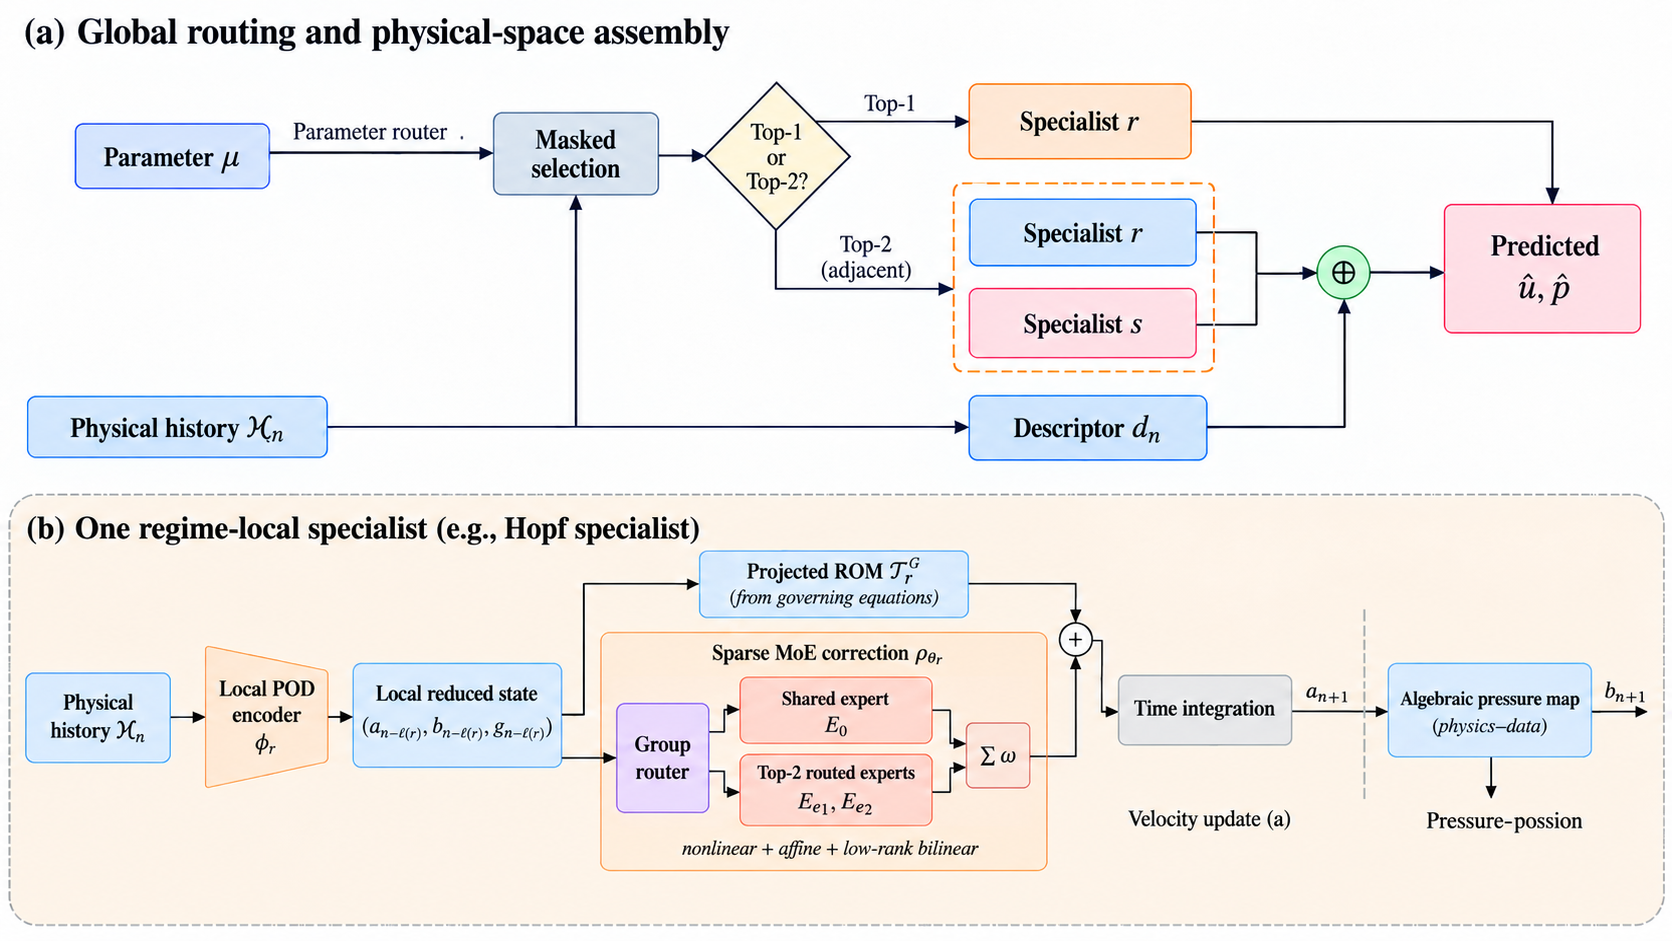
\includegraphics[width=\linewidth]{figures/ral_moe_rom_overview_user_20260908.png}
    \caption{
    Overview of RAL-MoE-ROM.
    (a) A parameter-only outer router selects one regime-local specialist or an adjacent pair. Selected specialists encode the same physical history in their native coordinates, evolve independently, and are combined only after reconstruction; recent physical history conditions the Top-2 fusion but not the outer router. (b) Each specialist augments the projected Galerkin backbone with a structured sparse MoE correction, while pressure is reconstructed algebraically. Flow thumbnails are schematic.
}
    \label{fig:ral_overview}
\end{figure}
\par

\section{Related Work}
\paragraph{Projection, learned dynamics, and autonomous rollout.}
POD--Galerkin methods project the governing equations onto a data-adapted basis and retain an explicit reduced dynamical system \citep{sirovich1987,berkooz1993,benner2015}. Their long-horizon accuracy can deteriorate when truncated interactions are not adequately represented, motivating closure and stabilization strategies
\citep{amsallem2012}. Non-intrusive reduced models instead infer reduced evolution laws directly from simulation data, ranging from projection-based operator inference to neural and latent-state dynamics
\citep{peherstorfer2016,hesthaven2018,champion2019,lee2020, pan2024domain,park2024}. Operator-inference methods provide a particularly direct connection between data-driven reduced dynamics and classical projection-based ROMs \citep{kramer2024}. Related neural-operator approaches learn mappings between function spaces
rather than explicit low-dimensional state evolution \citep{lu2021,kovachki2023}. Hybrid ROMs retain projected or physics-based structure while learning missing or unresolved reduced dynamics \citep{duraisamy2019,brunton2020,fresca2022,dar2023,geelen2023,manti2025}. RAL-MoE-ROM follows this hybrid principle, but places a structured sparse-MoE correction inside each regime-local ROM and trains the resulting specialist under closed-loop rollout, explicitly targeting autonomous multi-step prediction.




\paragraph{Localized representations and conditional dynamics.}
Local reduced bases, clustering strategies, localized operators, nonlinear manifolds, and parameter-space partitioning have been used to reduce the representational burden placed on a single global ROM \citep{amsallem2008,peherstorfer2014,kaiser2014,li2021cluster,diaz2024,bhat2025}. Recent work has further emphasized explicitly local reduced dynamics. In particular, ql-ROM partitions the solution manifold into clusters, constructs an intrusive ROM within each cluster, and connects the local models through assignment and change-of-basis operations
\citep{colanera2025}. These approaches motivate local reduced representations over restricted regions of parameter or state space, but they also introduce a coordination problem because independently constructed local models generally differ in
their mean fields, bases, scalings, and reduced operators. RAL-MoE-ROM addresses this issue differently: each reduced chart is paired with a complete autonomous specialist, the specialists retain independent coordinates during rollout, and cross-regime coupling is performed only after reconstruction in the common physical space. The resulting problem is therefore not merely one of selecting a local basis or switching between local coordinates, but of assembling independently evolved local dynamical systems.






\paragraph{Mixture-of-experts and cross-chart assembly.}
Classical hierarchical mixtures learn conditional expert assignments \citep{jacobs1991,jordan1994}, while sparse MoE architectures activate only a subset of experts for each input \citep{shazeer2017,fedus2022}. Many widely used MoE formulations specialize predictors or operator blocks that operate within a shared latent representation or a common output space. Recent work extends conditional specialization to physics-informed constraints, local implicit representations, neural-operator pretraining, and PDE forecasting \citep{ICLR2024_9aeda582,NEURIPS2024_b83fae17,NEURIPS2025_2d23a999,ICLR2026_754612bd}. These approaches demonstrate the value of conditional specialization, but they do not address the same cross-chart assembly problem considered here. RAL-MoE-ROM places conditional computation at two distinct levels: sparse experts operate within a single local coordinate system, while the outer routing level acts on complete local ROMs whose coordinates are constructed independently. When two local models are combined, they are evolved independently and
combined only after reconstruction in physical space, rather than by interpolating their reduced coefficients or operators. This distinction separates the present setting from standard within-representation MoE routing.

\section{RAL-MoE-ROM}
\label{sec:method}

RAL-MoE-ROM separates reduced modeling into three complementary components: regime-local representations, autonomous local specialists, and
cross-regime physical-space assembly. These components are organized by a two-level routing hierarchy. Overlapping regime-local parameter regions are equipped with independent reduced charts. Each chart supports a complete autonomous regime-local specialist that combines a projected ROM backbone with a structured sparse correction. The outer routing level then selects one specialist or an applicable adjacent pair and assembles only their reconstructed physical fields. Figure~\ref{fig:ral_overview} summarizes the overall construction; detailed
derivations are provided in Appendices~\ref{app:problem_pod}--\ref{app:routing}.

\subsection{Overlapping regime-local reduced charts}

Let $r\in\{S,H,P\}$ index steady, Hopf-onset, and periodic regimes, and let $\mathcal M_r$ denote the corresponding overlapping parameter regions. Each regime-local parameter region is equipped with its own reduced coordinate system. A physical velocity field is encoded and reconstructed as
\begin{equation}
  \bm a^{(r)}={\Phi_u^{(r)}}^{\top}M_u(\bm u-\bar{\bm u}^{(r)}),\qquad
  \widehat{\bm u}^{(r)}=\bar{\bm u}^{(r)}+\Phi_u^{(r)}\bm a^{(r)},
  \label{eq:main_chart}
\end{equation}
where $M_u$ is the finite-volume quadrature matrix. Gauge-corrected pressure is encoded analogously, yielding local coefficients
$\bm b^{(r)}$. 

A reduced chart comprises its mean fields, velocity and pressure bases, local coordinates, and normalization statistics. Each chart is associated with a regime-local parameter region and its own projected operators.
These quantities are constructed independently across regimes. Even when two charts have the same reduced dimension, their coordinates are not assumed to be componentwise aligned. Cross-regime assembly is consequently performed only after reconstruction in physical space.

\subsection{Regime-local hybrid specialists}

Within each chart, a projected Galerkin backbone describes the resolved dynamics, while a learned closure accounts for unresolved reduced dynamics:
\begin{equation}
  \dot{\bm a}^{(r)}=
  \underbrace{\bm c_r+\bm A_r\bm a^{(r)}+
  \bm H_r:\bigl(\bm a^{(r)}\otimes\bm a^{(r)}\bigr)+
  \bm C^p_r\bm b^{(r)}}_{\mathcal F_r^{G}(\bm a^{(r)},\bm b^{(r)};\mu)}
  +\bm\rho^u_{\theta_r}(\bm\xi^{(r)}).
  \label{eq:main_specialist}
\end{equation}
The learned term $\bm\rho^u_{\theta_r}$ is the velocity closure associated with chart $r$. Its input $\bm\xi^{(r)}$ collects standardized local state variables, the projected right-hand side, the physical parameter, and a short history of preceding states.

Separate sparse MoE maps are used for the velocity correction $\bm\rho^u_{\theta_r}$ and the learned pressure correction $\bm\rho^p_{\theta_r}$:
\begin{equation}
  \mathcal M^c_{\theta_r}(\bm\xi)=
  \omega^c_0 E^c_{0,m^\star}(\bm\xi)+
  \sum_{e\in\mathcal T_2^c}\omega^c_e E^c_{e,m^\star}(\bm\xi).
  \label{eq:main_inner_moe}
\end{equation}
Routing is hierarchical within each specialist. An expert group $m^\star$ is selected by a chart-local router or predetermined for a single-group or fixed-group specialist. Within that group, the velocity and pressure channels $c\in\{u,p\}$ independently select their two highest-scoring routed experts, while a shared expert remains active. The nonnegative weights $\omega_e^c$ are normalized over the active experts. Each active expert combines a nonlinear feature-conditioned branch with explicit linear and low-rank quadratic responses of the local reduced state; the exact parameterization is given in Appendix~\ref{app:specialists}.

After advancing velocity over one reduced time step, pressure is reconstructed algebraically as
\begin{equation}
  \bm b_{n+1}^{(r)}
  =\bm\gamma_n^{(r)}\odot\mathcal Q_r^{PP}(\bm a_{n+1}^{(r)};\mu)
  +\bm\rho^p_{\theta_r}(\bm\xi_n^{(r)}).
  \label{eq:main_pressure_closure}
\end{equation}
Here $\mathcal Q_r^{PP}$ denotes the chart-local reduced Pressure--Poisson map, $\bm\rho^p_{\theta_r}$ provides the learned pressure correction, and $\bm\gamma_n^{(r)} =\operatorname{sigmoid}(\bm\eta^p_{\theta_r}(\bm\xi_n^{(r)}))$ modulates the Pressure--Poisson contribution componentwise; $\odot$ denotes componentwise multiplication. Thus velocity is advanced dynamically, whereas pressure is reconstructed algebraically rather than evolved as a separate recurrent state.


\subsection{Closed-loop rollout training}

Each specialist is initialized from an encoded physical history and is then advanced recursively using its own predicted states. To expose the learned correction to the states encountered during autonomous rollout, training unrolls each specialist for $K$ steps and minimizes the
normalized coefficient error
\begin{equation}
  \mathcal L_r=\frac{1}{K}\sum_{k=1}^{K}\left[
  \frac{\left\|(\widehat{\bm a}_{n+k}^{(r)}-\bm a_{n+k}^{(r)})
  \oslash\bm\sigma_a^{(r)}\right\|_2^2}{d_u^{(r)}}
  +\frac{\left\|(\widehat{\bm b}_{n+k}^{(r)}-\bm b_{n+k}^{(r)})
  \oslash\bm\sigma_b^{(r)}\right\|_2^2}{d_p^{(r)}}\right].
  \label{eq:main_rollout_loss}
\end{equation}
Here $d_u^{(r)}$ and $d_p^{(r)}$ denote the chart-specific velocity and pressure coordinate dimensions, while $\bm\sigma_a^{(r)}$ and $\bm\sigma_b^{(r)}$ are scaling
vectors estimated from the corresponding regime-local training set; $\oslash$ denotes componentwise division. This coefficient-space objective is used for specialist training, whereas evaluation is performed on reconstructed physical fields. After initialization, no reference state from inside the prediction window is injected into the rollout. The chart-specific advancement rule is detailed in Appendix~\ref{app:specialists}, while rollout curricula and optimization settings are reported in Appendix~\ref{app:implementation}. Held-out trajectory splits are listed in Table~\ref{tab:chart_splits}.



\subsection{Cross-regime routing and physical-space T2-C assembly}

The outer E2 router receives only the standardized physical parameter $\widetilde\mu$ and returns a trajectory-level preference over the
regime-local specialists,
\[
\bm\pi(\mu)
=
\operatorname{softmax}\!\left(
\mathcal R_{E2}(\widetilde\mu)
\right).
\]
The probabilities are evaluated once and remain fixed throughout the rollout. The outer router does not use physical history. Chart-independent descriptors extracted from the initial history $\mathcal H_n$ enter only the T2-C gate described below.

A validation-supported applicability mask $m_r(\mathcal H_n,\mu,K)\in\{0,1\}$ marks whether specialist $r$ is applicable for the current parameter, initial history, and rollout horizon. The mask restricts the candidate set but does not modify the E2 probability
model itself. Under hard Top-1 routing, only the applicable specialist with the largest E2 probability is advanced.

When an adjacent pair is applicable ($S$--$H$ or $H$--$P$), both specialists are initialized from the same physical history, encoded in
their own coordinates, and advanced independently. Let $\bar\pi_r$ denote the E2 probability normalized over the selected pair. For reconstructed fields $\widehat{\bm q}^{(r)}$ and $\widehat{\bm q}^{(s)}$, T2-C predicts a history-conditioned logit correction to this pairwise preference and forms
\begin{equation}
  \widehat{\bm q}_{\rm T2C}(t)
  =\alpha\,\widehat{\bm q}^{(r)}(t)
  +(1-\alpha)\,\widehat{\bm q}^{(s)}(t),
  \qquad
  \alpha=
  \sigma\!\left(
  \operatorname{logit}(\bar\pi_r)+\Delta_\psi
  \right).
  \label{eq:main_t2c}
\end{equation}
Here $\Delta_\psi=c_\psi([\widetilde\mu;\bm d_n])$ is a learned logit correction based on the standardized parameter and the chart-independent physical-history descriptor $\bm d_n$, and $\sigma$ denotes the sigmoid. The scalar $\alpha$ is computed once for the prediction window and is shared by velocity and pressure. The field vector $\bm q$ collects reconstructed velocity and gauge-corrected pressure on the common physical mesh.

The two local trajectories remain independent throughout the rollout: fusion is applied only to their reconstructed outputs and is never fed back into either specialist. If no specialist is applicable, the method abstains from producing a ROM prediction. Applicability is determined empirically from validation support and should not be interpreted as a formal stability guarantee.

\section{Experiments}
\label{sec:experiments}

We organize the experiments around three questions: whether the regime-local specialists support autonomous prediction, whether
physical-space fusion improves prediction near regime transitions, and how the main local architectural choices affect prediction.
The three incompressible-flow benchmarks play complementary roles in answering these questions. All are two-dimensional systems in which varying the Reynolds number traverses steady, Hopf-onset, and periodic regimes. The circular-cylinder benchmark provides the local architecture ablation, the centered-square benchmark evaluates cross-regime routing and fusion in the $S$--$H$ and $H$--$P$ overlaps, and the fluidic-pinball benchmark provides the autonomous comparison with a classical POD--Galerkin ROM. Table~\ref{tab:benchmark_summary} summarizes the benchmark scope and roles. All splits are made at the level of complete parameter trajectories rather than individual snapshots or rollout windows; chart-wise parameter ranges and split counts are reported in Appendix~\ref{app:implementation}.

We report relative physical-field errors $E_u$ and $E_p$ in percent; their weighted definitions and benchmark-specific aggregation rules are given in Appendix~\ref{app:implementation}. For routing and fusion comparisons, $E_{\mathrm{joint}}=E_u+E_p$. The sum of displayed component errors can differ slightly from the reported joint error because values are rounded independently. A rollout window is labeled ``Divergent'' if it violates the predefined rollout-divergence criterion, either through a non-finite state or a
threshold violation. N/E denotes a setting that is not evaluable under this criterion; table-specific notes identify the cause.

\par
\begin{table}[H]
\centering
\caption{
Experimental scope and benchmark roles.
Local rank pairs $(r_u,r_p)$ and rollout horizons $K$ are ordered
$S,H,P$.
Additional overlap and periodic-core settings are specified in their
respective comparisons.
}
\label{tab:benchmark_summary}
\small
\setlength{\tabcolsep}{4pt}
\begin{tabular}{@{}>{\raggedright\arraybackslash}p{2.15cm}
>{\raggedright\arraybackslash}p{1.30cm}
>{\raggedright\arraybackslash}p{4.05cm}
>{\raggedright\arraybackslash}p{1.80cm}
>{\raggedright\arraybackslash}p{2.50cm}@{}}
\toprule
Benchmark & $Re$ range & Local ranks ($S,H,P$) & Rollout horizons & Primary role \\
\midrule
Circular cylinder
& 20--200
& $(32,32),\ (32,32),\ (32,32)$
& $56/56/48$
& Local architecture ablation \\
\addlinespace
Centered square
& 50--150
& $(5,4),\ (11,11),\ (28,26)$
& $16/48/24$
& Cross-regime routing/fusion \\
\addlinespace
Fluidic pinball
& 10--60
& $(4,3),\ (5,5),\ (17,16)$
& $56/56/32$
& Autonomous ROM baseline \\
\bottomrule
\end{tabular}
\end{table}
\par



\subsection{Do local specialists support accurate autonomous rollouts?}

We first examine whether the regime-local specialists maintain accurate predictions under autonomous rollout on the fluidic-pinball benchmark. Table~\ref{tab:pinball_autonomous} compares the learned specialists with a classical POD--Galerkin ROM over the Steady, Hopf, and Periodic regimes.

RAL-MoE-ROM achieves low physical-field errors across all four evaluation settings. In the Hopf and Periodic settings where POD--Galerkin errors are reported, the learned specialists consistently reduce both velocity and pressure
errors, with the largest differences appearing in pressure. For example, the Hopf joint error decreases from $48.94\%$ to $2.085\%$, while the standard Periodic error decreases from $43.20\%$ to $0.8415\%$. The longer-horizon Periodic-core evaluation shows the same trend, with $E_{\mathrm{joint}}$ reduced from $41.91\%$ to $1.672\%$. Together, these results show that the learned specialists maintain low physical-field error over the evaluated autonomous horizons.

\par
\begin{table}[H]
\centering
\caption{
Autonomous local-specialist prediction on the fluidic-pinball benchmark. Errors are physical-field percentages; lower is better. Periodic-core denotes the longer-horizon periodic evaluation; complete protocol details are given in Appendix~\ref{app:pinball}. A dash indicates that no baseline error is reported.
}
\label{tab:pinball_autonomous}
\small
\setlength{\tabcolsep}{5pt}
\begin{tabular}{@{}llrrr@{}}
\toprule
Evaluation setting & Model & $E_u$ & $E_p$ & $E_{\mathrm{joint}}$ \\
\midrule
Steady ($K=56$)
& POD--Galerkin
& -- & -- & -- \\
& RAL-MoE-ROM
& 0.2247 & 0.7593 & 0.9840 \\
\addlinespace

Hopf ($K=56$)
& POD--Galerkin
& 0.4378 & 48.50 & 48.94 \\
& RAL-MoE-ROM
& 0.0995 & 1.986 & 2.085 \\
\addlinespace

Periodic ($K=32$)
& POD--Galerkin
& 1.641 & 41.56 & 43.20 \\
& RAL-MoE-ROM
& 0.2897 & 0.5518 & 0.8415 \\
\addlinespace

Periodic-core ($K=56$)
& POD--Galerkin
& 2.555 & 39.36 & 41.91 \\
& RAL-MoE-ROM
& 0.6222 & 1.050 & 1.672 \\
\bottomrule
\end{tabular}
\end{table}
\par

A complementary POD--DeepONet experiment further separates one-step prediction from autonomous rollout.
The model attains $E_u=1.5921\%$ and $E_p=23.3447\%$ on 4,228 held-out one-step pairs, but only one of 28 held-out trajectories completes the prescribed autonomous rollout evaluation. Because its temporal cadence differs from that of the Periodic specialist, we use this result only to contrast one-step prediction with autonomous rollout, rather than as a matched long-horizon accuracy comparison (Appendix~\ref{app:pinball}).





\subsection{Does physical-space fusion improve prediction in regime overlaps?}
To evaluate the second routing level while holding the local specialists fixed, we compare the centered-square $S$--$H$ and $H$--$P$ overlaps at $K=24$ (Table~\ref{tab:routing_fusion}). We compare hard E2 Top-1 routing with two simple fusion rules, the Equal blend and the E2-probability blend, together with the learned T2-C gate; a diagnostic convex oracle provides an a posteriori reference. To test whether T2-C benefits specifically from physical-history information, we additionally include an architecture-matched T2-C $\mu$-only ablation. The same gate architecture and optimization protocol are retained, but the standardized history-descriptor channels are set to zero. This preserves the gate parameterization and trainable parameter count while removing history information.


The $\mu$-only ablation reveals that parameter conditioning alone has overlap-dependent value. For $S$--$H$, its joint error is essentially unchanged relative to the E2-probability blend ($2.1846\%$ versus $2.1847\%$), whereas for $H$--$P$ it improves the same baseline from $1.6618\%$ to $1.1504\%$. Adding the physical-history descriptor improves both overlaps further, reducing $E_{\mathrm{joint}}$ to $1.1958\%$ and $0.8465\%$, respectively. Relative to the a posteriori best fixed-specialist reference, full T2-C reduces joint error by $30.9\%$ on $S$--$H$ and $29.9\%$ on $H$--$P$. Relative to the deployable E2 Top-1 router, the corresponding reductions are $30.9\%$ and $54.2\%$. The validation-selected T2-C errors are also close to the diagnostic convex oracle in both overlaps. Representative reconstructed fields and velocity-error maps are shown in Figure~\ref{fig:square_overlap}.

Across three paired gate-training seeds, full T2-C outperforms the architecture-matched $\mu$-only gate in every run for both overlaps.
Across the three paired runs, the mean reduction relative to $\mu$-only is $45.3\%$ for $S$--$H$ and $26.2\%$ for $H$--$P$. Full T2-C yields
$E_{\mathrm{joint}}=1.1957\pm0.0001\%$ on $S$--$H$ and $0.8500\pm0.0035\%$ on $H$--$P$, where $\pm$ denotes the sample standard
deviation across the three gate-training seeds. Only gate training is repeated across seeds; the specialists, E2 router, candidate rollouts, data splits, normalization, and optimization protocol are fixed. These statistics therefore characterize gate-training variability rather than full-pipeline uncertainty. Component-wise errors and seed-level results are reported in Appendix~\ref{app:square}, with the corresponding fluidic-pinball overlap study in Appendix~\ref{app:pinball}.


\par
\begin{table}[H]
\centering
\caption{
Validation-selected cross-regime routing and fusion on the centered-square benchmark at $K=24$. Entries are terminal-step $E_{\mathrm{joint}}$ (\%); lower is better. T2-C $\mu$-only uses the same gate architecture with all standardized history-descriptor channels set to zero. The oracle is an a posteriori convex reference and is not available at inference. Three-seed gate-training variability is reported separately in
Appendix~\ref{app:square}. Bold marks the best deployable method in this validation-selected comparison.
}
\label{tab:routing_fusion}
\small
\setlength{\tabcolsep}{3.5pt}
\begin{threeparttable}
\begin{tabular}{@{}lrrrrrrr@{}}
\toprule
Overlap & Best fixed$^\ast$ & E2 Top-1 & \shortstack{Equal\\blend} & \shortstack{E2-probability\\blend} & \shortstack{T2-C\\$\mu$-only} & T2-C & \shortstack{Convex\\oracle}\\
\midrule
$S$--$H$ & 1.7298 & 1.7298 & 3.0321 & 2.1847 & 2.1846 & \textbf{1.1958} & 1.1842 \\
$H$--$P$ & 1.2079 & 1.8473 & 1.6146 & 1.6618 & 1.1504 & \textbf{0.8465} & 0.8384 \\
\bottomrule
\end{tabular}
\begin{tablenotes}[flushleft]
\footnotesize
\item[$\ast$] Best fixed denotes the a posteriori fixed-specialist reference selected by aggregate evaluation error over the corresponding overlap (Hopf for $S$--$H$, Periodic for $H$--$P$). It is not a routing strategy available at inference.
\end{tablenotes}
\end{threeparttable}
\end{table}
\par

\par
\begin{figure}[H]
\centering
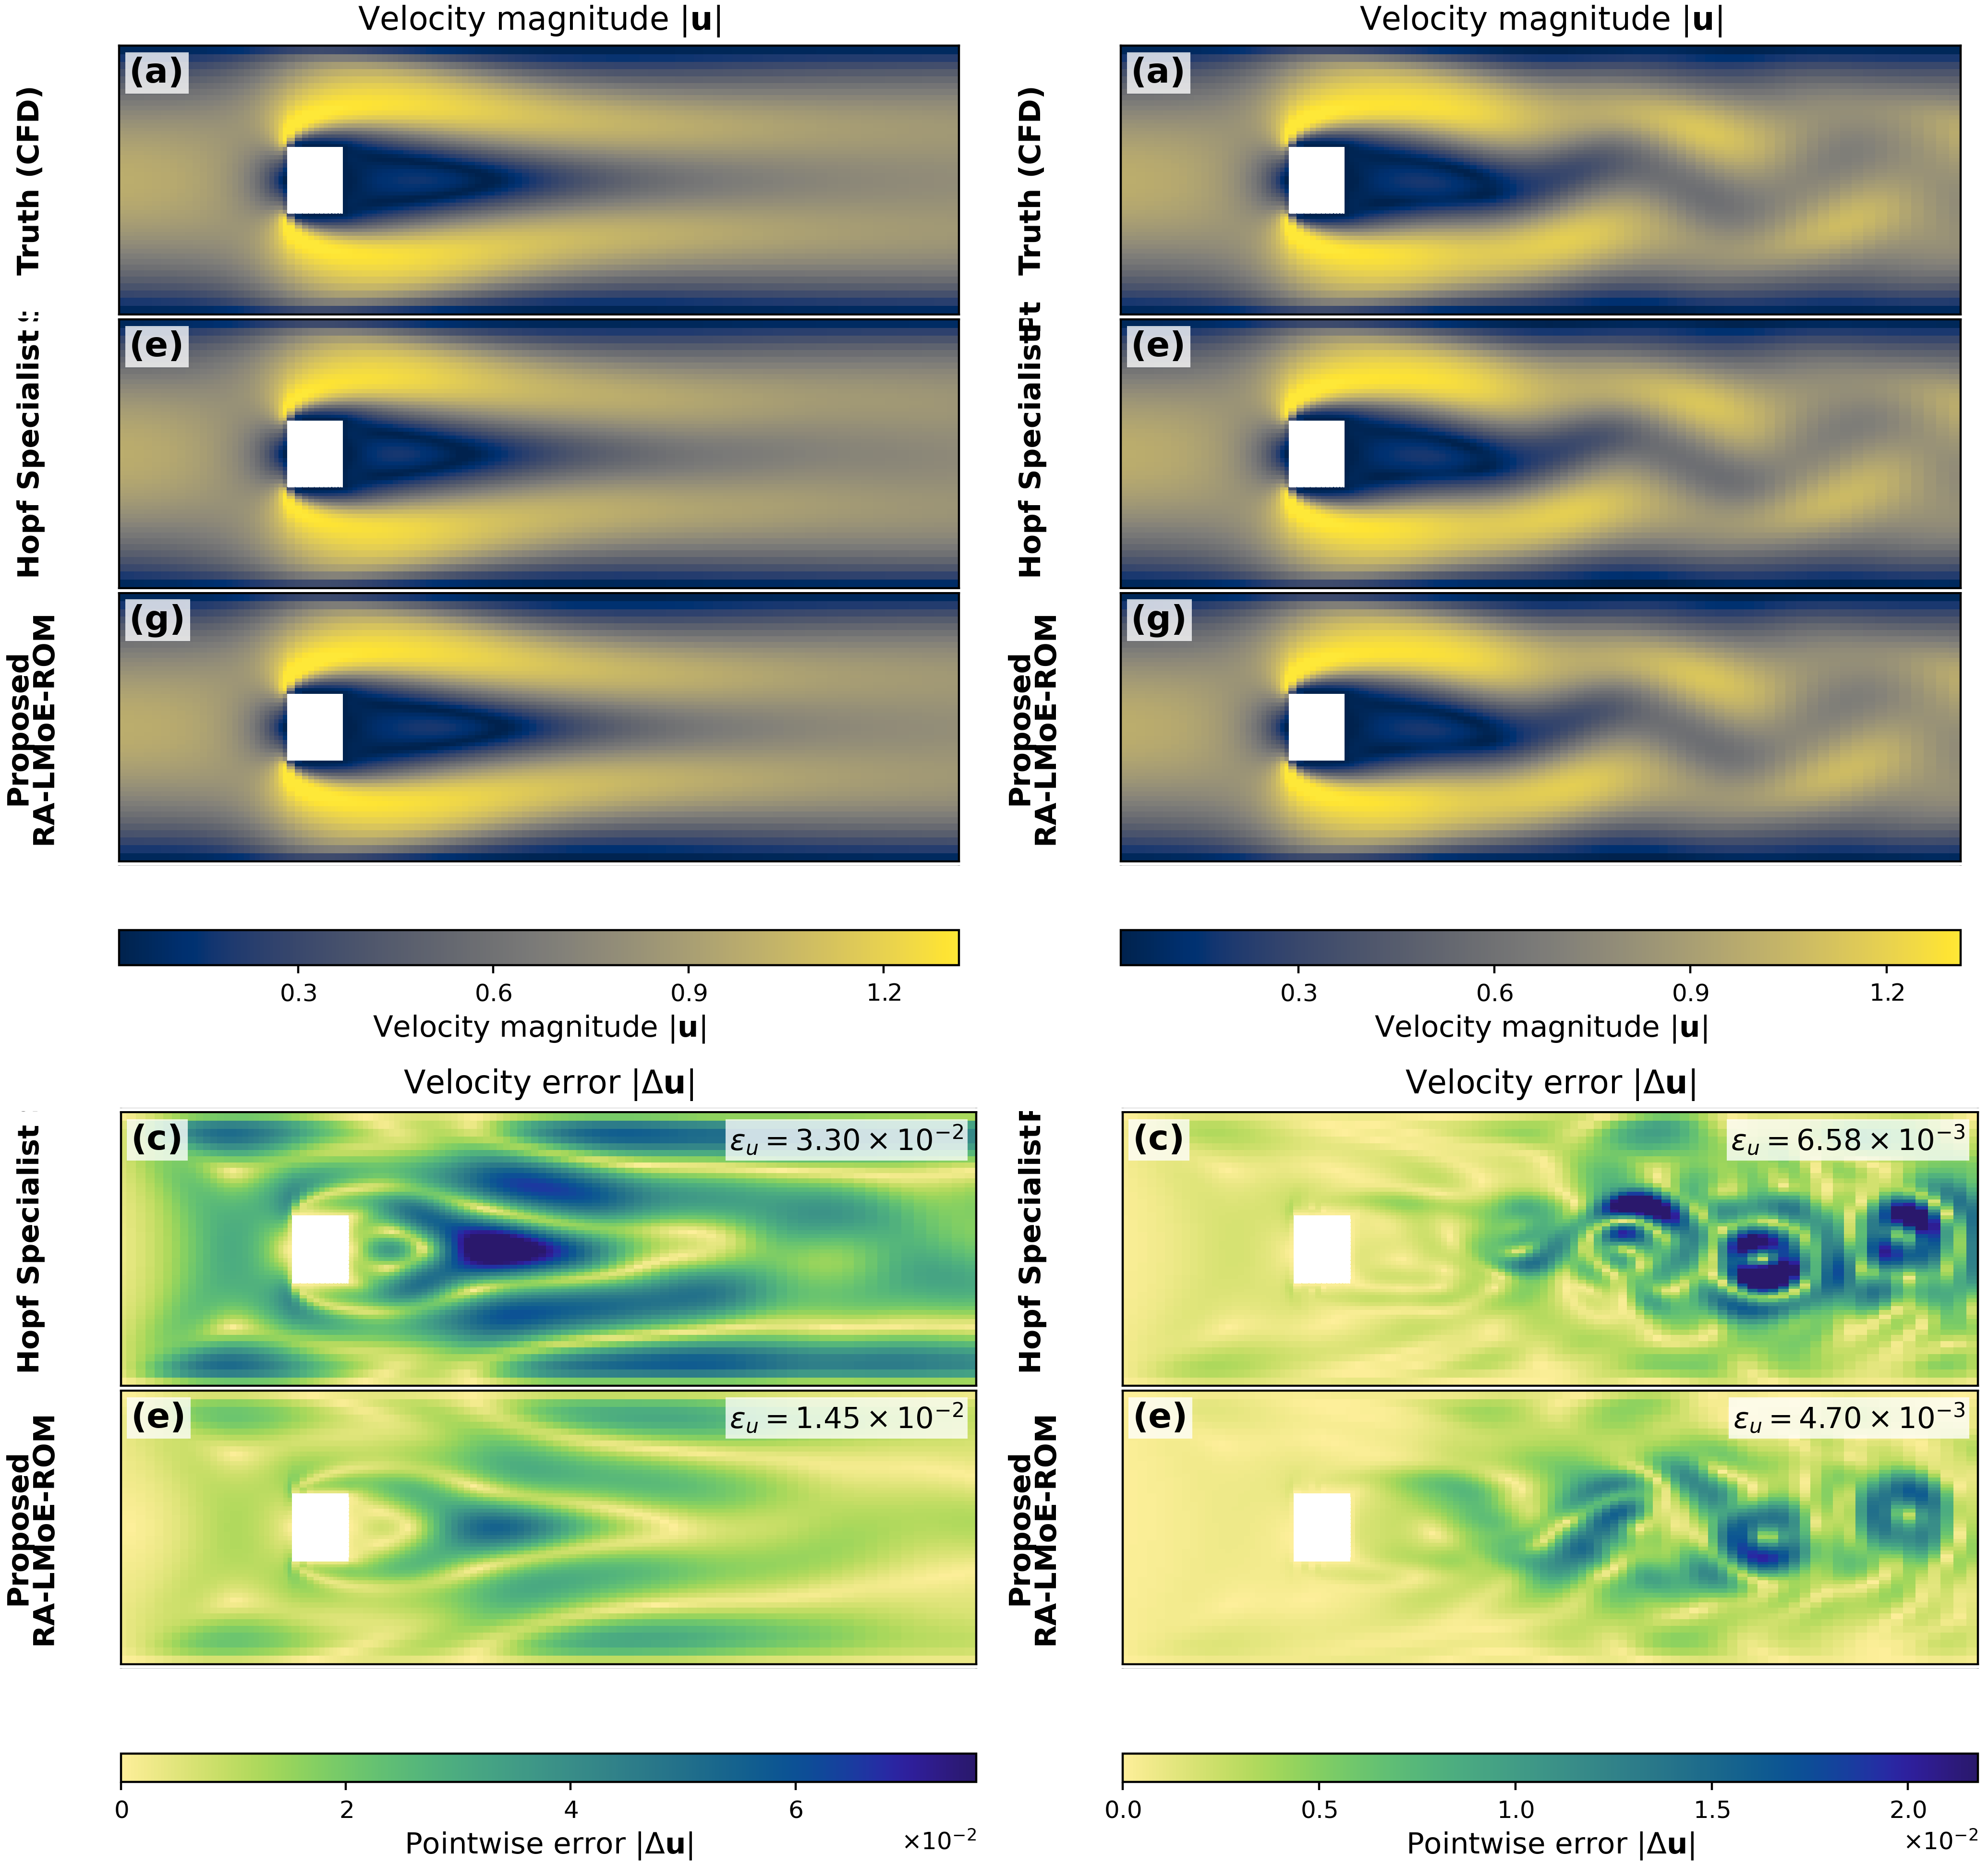
\includegraphics[width=\linewidth]{figures/square_overlap_compact.png}
\caption{Representative centered-square overlap predictions for $S$--$H$ (left) and $H$--$P$ (right). T2-C combines independently evolved local predictions only after reconstruction in physical space. The displayed examples illustrate the corresponding reduction in velocity-field error; complete velocity and pressure comparisons are reported in Appendix~\ref{app:square}.
}
\label{fig:square_overlap}
\end{figure}
\par



\subsection{How do local architectural choices affect prediction?}

The circular-cylinder benchmark is used to examine three local architectural choices: structured expert parameterization, the projected ROM backbone, and regime localization (Table~\ref{tab:circular_full_reorg}). Vanilla-FNN-MoE retains the regime-local setting but replaces the structured expert map with conventional feed-forward experts. DataOnly-MoE removes the projected Galerkin and Pressure--Poisson backbone, leaving the learned local dynamics to account for the evolution from data. Global MoE replaces the regime-local charts and specialists with a single global reduced representation and dynamical model. All comparisons are reported in physical-field error so that models with different reduced coordinates are assessed in a common physical space. These comparisons characterize architectural effects under the available fixed models rather than parameter-matched capacity controls. Total and active trainable parameter counts for the analyzed Hopf and Periodic specialists are reported in Appendix~\ref{app:parameter_counts}.

\begin{table}[H]
\centering
\caption{Circular-cylinder autonomous-rollout errors (\%). A dash indicates that the rollout diverged.}
\label{tab:circular_full_reorg}
\small
\setlength{\tabcolsep}{4pt}
\begin{tabular}{llcc}
\toprule
Regime & Model & $E_u$ & $E_p$ \\
\midrule
Steady ($K=56$)
& RAL-MoE-ROM & 0.1027 & 0.7875 \\
& Vanilla-FNN-MoE & 0.1690 & 10.3883 \\
& DataOnly-MoE & 0.3380 & - \\
& Global MoE & 0.2125 & 4.4795 \\
\midrule
Hopf ($K=56$)
& RAL-MoE-ROM & 0.0160 & 0.1338 \\
& Vanilla-FNN-MoE & - & - \\
& DataOnly-MoE & 0.2570 & - \\
& Global MoE & 0.0189 & 0.1721 \\
\midrule
Periodic ($K=48$)
& RAL-MoE-ROM & 0.7412 & 3.8213 \\
& Vanilla-FNN-MoE & 2.0615 & 8.6458 \\
& DataOnly-MoE & 1.3266 & 6.5350 \\
& Global MoE & 0.8800 & 4.2731 \\
\bottomrule
\end{tabular}
\end{table}
















Replacing the structured expert map with conventional feed-forward experts increases both velocity and pressure errors in the Steady and Periodic regimes; the Vanilla-FNN-MoE Hopf model is not evaluable under the prescribed rollout criterion. Removing the projected ROM backbone produces the largest degradation, with particularly large pressure errors for DataOnly-MoE in the Steady and Hopf regimes. Among the ablations, Global MoE provides the closest overall comparison and is particularly close to the full model in the Hopf regime. Nevertheless, the regime-local specialists retain lower reported physical-field errors in all three regimes. Together, these comparisons support the roles of structured expert corrections, the projected ROM backbone, and regime-local representations under the tested architectures. They are not parameter-matched capacity controls. Cross-regime assembly is evaluated separately in Table~\ref{tab:routing_fusion}. Additional post-hoc internal-routing diagnostics are reported in
Appendix~\ref{app:internal_routing}.




\FloatBarrier
\section{Conclusion}

We introduced RAL-MoE-ROM, a hierarchical reduced-order modeling framework that separates within-regime dynamical specialization from cross-regime assembly. Regime-local ROMs retain independent reduced coordinates and augment projected dynamics with structured sparse corrections, while
cross-regime coupling is performed only after reconstruction in physical space. Across three parameterized incompressible-flow benchmarks, the local specialists support accurate autonomous rollouts, and history-conditioned T2-C improves prediction in the evaluated regime overlaps. The present study assumes a validation-supported regime coverage and evaluates pairwise fusion only for adjacent specialists on two-dimensional incompressible flows. Future work will investigate learned regime discovery, constraint-preserving physical-space assembly, and higher-dimensional dynamical systems.


\subsubsection*{Reproducibility statement}
The main text reports the benchmark roles, evaluation horizons, baselines, and metrics. Appendices~A--E document the local-coordinate construction, projected operators, specialist architecture, routing and fusion procedure, and implementation details. Appendices~F--H provide benchmark-specific results.
Appendix~\ref{app:internal_routing} reports post-hoc internal-routing statistics
from fixed validation-selected Hopf and Periodic specialists on held-out
rollout windows; these diagnostics are not used for model selection.
Appendix~\ref{app:square} additionally reports an architecture-matched descriptor
ablation and three-seed variability of the centered-square T2-C gate, with the
underlying specialists and E2 router held fixed.

\subsection*{AI use statement}
% Authors must confirm this disclosure against the final submission workflow.
Generative AI tools, including ChatGPT and Codex, were used solely to assist with language polishing and LaTeX formatting. The authors take full responsibility for reviewing and verifying all scientific
content, mathematical formulations, experimental configurations, numerical
results, and conclusions, and for the final manuscript and all reported results.

\bibliography{references,legacy_references}
\bibliographystyle{iclr2027_conference}

\appendix
\section{Full problem setup and weighted POD construction}
\label{app:problem_pod}

\subsection{Parameterized full-order model, gauge, and regime coverage}

After spatial discretization, the velocity
$\bm u(t;\mu)\in\mathbb R^{N_u}$ and pressure
$p(t;\mu)\in\mathbb R^{N_p}$ satisfy
\begin{equation}
    \dot{\bm u}
    =
    \bm f_h(\mu)
    +\mathcal L_h(\mu)\bm u
    -\mathcal N_h(\bm u,\bm u;\mu)
    -\nabla_h(\mu)p,
    \qquad
    \operatorname{div}_h(\mu)\bm u=0.
    \label{eq:app_fom}
\end{equation}
Pressure is defined only up to an additive constant.
With positive finite-volume weights $\bm w$, each pressure snapshot is mapped
to the weighted zero-mean gauge
\begin{equation}
    \Gamma_p(q)
    =
    q-\frac{\bm w^\top q}{\bm w^\top\bm 1}\bm 1,
    \qquad
    p^\circ=\Gamma_p(p),
    \qquad
    \bm w^\top p^\circ=0.
    \label{eq:app_pressure_gauge}
\end{equation}

The parameter domain is covered by overlapping regime-local parameter regions,
\begin{equation}
    \mathcal M
    \subseteq
    \bigcup_{r\in\{S,H,P\}}\mathcal M_r,
    \qquad
    \mathcal O_{SH}
    =
    \mathcal M_S\cap\mathcal M_H,
    \qquad
    \mathcal O_{HP}
    =
    \mathcal M_H\cap\mathcal M_P,
    \label{eq:app_regime_cover}
\end{equation}
where $S$, $H$, and $P$ denote the steady, Hopf-onset, and periodic
regimes, respectively.
Only adjacent overlaps are used; no direct $S$--$P$ overlap is considered.


\subsection{Area-weighted local POD}

The finite-volume quadrature induces the weighted inner products
\begin{equation}
    \langle\bm v,\bm z\rangle_{M_u}
    =
    \bm v^\top M_u\bm z,
    \qquad
    \langle q,s\rangle_{M_p}
    =
    q^\top M_p s,
    \qquad
    M_p=\operatorname{diag}(\bm w),
    \qquad
    M_u=\operatorname{diag}(M_p,M_p).
    \label{eq:app_weighted_inner_products}
\end{equation}

For chart $r$, let $d_u^{(r)}$ and $d_p^{(r)}$ denote the retained velocity
and pressure dimensions.
Let $X_u^{(r)}$ and $X_p^{(r)}$ collect the centered velocity and
gauge-corrected pressure snapshots from the training trajectories assigned
to that chart.
The corresponding chart-specific means are denoted by
$\bar{\bm u}^{(r)}$ and $\bar p^{(r),\circ}$.
The local POD bases solve
\begin{align}
    \Phi_u^{(r)}
    &\in
    \underset{\Psi^\top M_u\Psi=I_{d_u^{(r)}}}
    {\operatorname{arg\,min}}
    \left\|
        X_u^{(r)}
        -\Psi\Psi^\top M_uX_u^{(r)}
    \right\|_{M_u,F}^2,
    \\
    \Phi_p^{(r)}
    &\in
    \underset{\Psi^\top M_p\Psi=I_{d_p^{(r)}}}
    {\operatorname{arg\,min}}
    \left\|
        X_p^{(r)}
        -\Psi\Psi^\top M_pX_p^{(r)}
    \right\|_{M_p,F}^2,
    \label{eq:app_pod_optimization}
\end{align}
where
\begin{equation}
    \|Y\|_{M,F}^2=\operatorname{tr}(Y^\top MY).
\end{equation}

Equivalently, consider the weighted singular value decompositions
\begin{equation}
    M_u^{1/2}X_u^{(r)}
    =
    U_u^{(r)}\Sigma_u^{(r)}{V_u^{(r)}}^\top,
    \qquad
    M_p^{1/2}X_p^{(r)}
    =
    U_p^{(r)}\Sigma_p^{(r)}{V_p^{(r)}}^\top.
\end{equation}
The retained bases are
\begin{equation}
    \Phi_u^{(r)}
    =
    M_u^{-1/2}
    U_u^{(r)}(:,1{:}d_u^{(r)}),
    \qquad
    \Phi_p^{(r)}
    =
    M_p^{-1/2}
    U_p^{(r)}(:,1{:}d_p^{(r)}),
    \label{eq:app_weighted_svd_bases}
\end{equation}
and satisfy
\begin{equation}
    {\Phi_u^{(r)}}^\top M_u\Phi_u^{(r)}=I,
    \qquad
    {\Phi_p^{(r)}}^\top M_p\Phi_p^{(r)}=I.
\end{equation}
Because the pressure snapshots and their chart mean satisfy the same weighted
gauge condition, the pressure basis also satisfies
\begin{equation}
    \bm w^\top\Phi_p^{(r)}=\bm 0^\top .
\end{equation}

Encoding and decoding are performed independently within each chart:
\begin{align}
    \bm a^{(r)}
    &=
    {\Phi_u^{(r)}}^\top
    M_u
    \bigl(\bm u-\bar{\bm u}^{(r)}\bigr),
    &
    \mathcal D_r^u(\bm a^{(r)})
    &=
    \bar{\bm u}^{(r)}
    +\Phi_u^{(r)}\bm a^{(r)},
    \\
    \bm b^{(r)}
    &=
    {\Phi_p^{(r)}}^\top
    M_p
    \bigl(\Gamma_p(p)-\bar p^{(r),\circ}\bigr),
    &
    \mathcal D_r^p(\bm b^{(r)})
    &=
    \bar p^{(r),\circ}
    +\Phi_p^{(r)}\bm b^{(r)}.
    \label{eq:app_encode_decode}
\end{align}

The reduced coefficients are standardized using chart-local statistics
estimated from the corresponding training trajectories:
\begin{equation}
    \widetilde{\bm a}^{(r)}
    =
    \bigl(
        \bm a^{(r)}-\bm\mu_a^{(r)}
    \bigr)
    \oslash
    \bm\sigma_a^{(r)},
    \qquad
    \widetilde{\bm b}^{(r)}
    =
    \bigl(
        \bm b^{(r)}-\bm\mu_b^{(r)}
    \bigr)
    \oslash
    \bm\sigma_b^{(r)}.
    \label{eq:app_local_scalers}
\end{equation}
Additional specialist features and their normalization are specified in
Appendix~\ref{app:specialists}.

All chart-local means, POD bases, and scaling statistics are constructed
independently.
Consequently, reduced coefficient vectors from different charts are not
assumed to be componentwise comparable; only their decoded physical fields lie in a common physical comparison space.






\section{Projected Galerkin and pressure operators}
\label{app:rom}

\subsection{Chart-local Galerkin momentum dynamics}

For each chart $r\in\{S,H,P\}$, substituting the chart-local affine reconstructions
from Appendix~\ref{app:problem_pod} into the semi-discrete
momentum equation and testing against the local velocity basis yields
\begin{equation}
    \dot{\bm a}^{(r)}
    =
    \bm c_r(\mu)
    +
    A_r(\mu)\bm a^{(r)}
    +
    H_r(\mu):
    \bigl(
        \bm a^{(r)}\otimes\bm a^{(r)}
    \bigr)
    +
    C_r^p(\mu)\bm b^{(r)}.
    \label{eq:app_projected_momentum}
\end{equation}
Here ``$:$'' denotes the double contraction.
For velocity modes
$\bm\phi_i^{u,(r)}$,
$i=1,\ldots,d_u^{(r)}$,
and pressure modes
$\phi_\ell^{p,(r)}$,
$\ell=1,\ldots,d_p^{(r)}$,
the projected operators are
\begin{align}
    [\bm c_r(\mu)]_i
    &=
    \Bigl\langle
        \bm\phi_i^{u,(r)},
        \bm f_h(\mu)
        +
        \mathcal L_h(\mu)\bar{\bm u}^{(r)}
        -
        \mathcal N_h
        \bigl(
            \bar{\bm u}^{(r)},
            \bar{\bm u}^{(r)};
            \mu
        \bigr)
        -
        \nabla_h(\mu)\bar p^{(r),\circ}
    \Bigr\rangle_{M_u},
    \\
    [A_r(\mu)]_{ij}
    &=
    \Bigl\langle
        \bm\phi_i^{u,(r)},
        \mathcal L_h(\mu)\bm\phi_j^{u,(r)}
        -
        \mathcal N_h
        \bigl(
            \bar{\bm u}^{(r)},
            \bm\phi_j^{u,(r)};
            \mu
        \bigr)
        -
        \mathcal N_h
        \bigl(
            \bm\phi_j^{u,(r)},
            \bar{\bm u}^{(r)};
            \mu
        \bigr)
    \Bigr\rangle_{M_u},
    \\
    [H_r(\mu)]_{ijk}
    &=
    -
    \Bigl\langle
        \bm\phi_i^{u,(r)},
        \mathcal N_h
        \bigl(
            \bm\phi_j^{u,(r)},
            \bm\phi_k^{u,(r)};
            \mu
        \bigr)
    \Bigr\rangle_{M_u},
    \\
    [C_r^p(\mu)]_{i\ell}
    &=
    -
    \Bigl\langle
        \bm\phi_i^{u,(r)},
        \nabla_h(\mu)\phi_\ell^{p,(r)}
    \Bigr\rangle_{M_u}.
    \label{eq:app_projected_operators}
\end{align}

We denote the resulting chart-local projected momentum vector field by
\begin{equation}
    \mathcal F_r^G
    \bigl(
        \bm a^{(r)},
        \bm b^{(r)};
        \mu
    \bigr)
    =
    \bm c_r(\mu)
    +
    A_r(\mu)\bm a^{(r)}
    +
    H_r(\mu):
    \bigl(
        \bm a^{(r)}\otimes\bm a^{(r)}
    \bigr)
    +
    C_r^p(\mu)\bm b^{(r)}.
    \label{eq:app_galerkin_backbone}
\end{equation}
This vector field provides the explicit projected Galerkin backbone of the
regime-local specialist introduced in
Eq.~(\plaineqref{eq:main_specialist}).


\subsection{Gauge-consistent pressure--Poisson map}

The pressure component is represented through a chart-local
Pressure--Poisson relation.
At the continuous level, the gauge-corrected pressure satisfies
\begin{equation}
    -\Delta p^\circ
    =
    \nabla\!\cdot
    \left[
        (\bm u\!\cdot\!\nabla)\bm u
        -
        \bm f
    \right],
    \qquad
    \int_\Omega p^\circ\,\mathrm d\Omega=0,
    \label{eq:app_continuous_pressure_poisson}
\end{equation}
with boundary conditions inherited from the momentum equation.
After discretization, substitution of the chart-local affine velocity
representation, and projection onto the local pressure basis, the reduced
pressure coefficients satisfy
\begin{equation}
    K_r^p(\mu)\bm b^{PP,(r)}
    =
    \bm d_r(\mu)
    +
    B_r(\mu)\bm a^{(r)}
    +
    Q_r(\mu):
    \bigl(
        \bm a^{(r)}\otimes\bm a^{(r)}
    \bigr).
    \label{eq:app_pressure_poisson_system}
\end{equation}
The corresponding chart-local Pressure--Poisson map is therefore
\begin{equation}
    \mathcal Q_r^{PP}
    \bigl(
        \bm a^{(r)};
        \mu
    \bigr)
    =
    [K_r^p(\mu)]^{-1}
    \left[
        \bm d_r(\mu)
        +
        B_r(\mu)\bm a^{(r)}
        +
        Q_r(\mu):
        \bigl(
            \bm a^{(r)}\otimes\bm a^{(r)}
        \bigr)
    \right].
    \label{eq:app_pressure_poisson_map}
\end{equation}

Because the pressure basis lies in the weighted zero-mean subspace defined in
Appendix~\ref{app:problem_pod}, the constant-pressure null direction is
removed before projection.
Thus $\mathcal Q_r^{PP}$ produces pressure coefficients in the native
coordinates of chart $r$ without introducing an additional cross-chart
pressure gauge.

The pair
\begin{equation}
    \left(
        \mathcal F_r^G,
        \mathcal Q_r^{PP}
    \right)
\end{equation}
is constructed independently for each regime-local chart.
Accordingly, each chart carries its own parameter region, mean fields,
POD bases, coefficient scalings, projected momentum operators, and
Pressure--Poisson map.
These chart-local operators are used only within their native reduced
coordinates; no componentwise interpolation of reduced states or projected
operators is assumed across charts.


\section{Regime-local specialist architecture and closed-loop training}
\label{app:specialists}

For each regime-local chart $r$, we define a self-contained 
specialist in its native reduced coordinates: velocity is advanced
dynamically, whereas pressure is reconstructed algebraically.
The projected operators from Appendix~\ref{app:rom} provide the underlying physics, while learned terms model unresolved reduced dynamics. The velocity coefficients satisfy
\begin{equation}
  \dot{\bm a}^{(r)}
  =
  \mathcal F_r^G
  \left(
    \bm a^{(r)},\bm b^{(r)};\mu
  \right)
  +
  \bm\rho^u_{\theta_r}
  \left(
    \bm\xi^{(r)}
  \right).
  \label{eq:app_hybrid_velocity_rhs}
\end{equation}
After each reduced velocity time step, pressure is reconstructed through
\begin{align}
  \bm b_{n+1}^{PP,(r)}
  &=
  \mathcal Q_r^{PP}
  \left(
    \bm a_{n+1}^{(r)};\mu
  \right),
  \nonumber\\
  \bm\gamma_n^{(r)}
  &=
  \operatorname{sigmoid}
  \left(
    \bm\eta^p_{\theta_r}
    (\bm\xi_n^{(r)})
  \right),
  \nonumber\\
  \bm b_{n+1}^{(r)}
  &=
  \bm\gamma_n^{(r)}
  \odot
  \bm b_{n+1}^{PP,(r)}
  +
  \bm\rho^p_{\theta_r}
  (\bm\xi_n^{(r)}),
  \qquad
  \bm\gamma_n^{(r)}
  \in(0,1)^{d_p^{(r)}}.
  \label{eq:app_pressure_closure}
\end{align}
The gate modulates the projected Pressure--Poisson contribution, while
$\bm\rho^p_{\theta_r}$ provides the learned pressure correction.


\subsection{Features and structured sparse experts}

Let
\begin{equation}
  \bm g_n^{(r)}
  =
  \mathcal F_r^G
  \left(
    \bm a_n^{(r)},\bm b_n^{(r)};\mu
  \right)
  \label{eq:app_galerkin_feature}
\end{equation}
denote the projected velocity right-hand side defined in Eq.~(\plaineqref{eq:app_galerkin_backbone}). The specialist uses the ordered three-state history
\begin{equation}
  \mathcal H_n^{(r)}
  =
  \left(
    \bm a_{n-\ell}^{(r)},
    \bm b_{n-\ell}^{(r)},
    \bm g_{n-\ell}^{(r)}
  \right)_{\ell=0}^{2},
  \label{eq:app_specialist_history}
\end{equation}
and constructs
\begin{equation}
  \bm\xi_n^{(r)}
  =
  \operatorname{Feat}_r
  \left(
    \mathcal H_n^{(r)},\mu
  \right),
  \qquad
  \bm z_n^{(r)}
  =
  \operatorname{Enc}_r
  \left(
    \bm\xi_n^{(r)}
  \right).
  \label{eq:app_specialist_features}
\end{equation}
The feature map contains standardized local states, projected
right-hand sides and parameter features. All normalization statistics are estimated from the corresponding chart-specific training set. Internal routing first selects an expert group. When group selection is learned,
\begin{equation}
  m^\star
  =
  \underset{m\in\mathcal G_r}{\operatorname{arg\,max}}
  \;
  \pi_{r,m}^{\mathrm{grp}}
  \left(
    \bm z_n^{(r)},\bm\xi_n^{(r)}
  \right),
  \label{eq:app_group_top1}
\end{equation}
whereas $m^\star$ is predetermined for single-group or fixed-group
specialists. Within the selected group, velocity and pressure use separate channel routers. For $c\in\{u,p\}$, let $\mathcal T_2^c$ denote the two routed experts with the largest channel-specific weights. Together with the shared expert $e=0$,
\begin{equation}
  \mathcal M_{\theta_r}^c
  =
  \omega_0^c
  E_{0,m^\star}^c
  +
  \sum_{e\in\mathcal T_2^c}
  \omega_e^c
  E_{e,m^\star}^c,
  \qquad
  \omega_e^c\ge0,
  \qquad
  \omega_0^c+\sum_{e\in\mathcal T_2^c}\omega_e^c=1.
  \label{eq:app_channel_sparse_moe}
\end{equation}
The two channel mixtures define the velocity and pressure corrections
$\bm\rho_{\theta_r}^u$ and $\bm\rho_{\theta_r}^p$, respectively. The explicit linear and quadratic branches operate on the channel-specific reduced-state inputs
\begin{equation}
  \bm s^{u,(r)}
  =
  \widetilde{\bm a}^{(r)},
  \qquad
  \bm s^{p,(r)}
  =
  \operatorname{col}
  \left(
    \widetilde{\bm a}^{(r)},
    \widetilde{\bm b}^{(r)}
  \right).
  \label{eq:app_expert_state_slices}
\end{equation}
For output component $j$, each expert is
\begin{align}
  \left[E_{e,m}^c\right]_j
  &=
  \left[
    N_{e,m}^c
    \left(
      \bm z,\bm s^c
    \right)
  \right]_j
  +
  \left[
    W_{e,m}^{c,\mathrm{lin}}
    \bm s^c
  \right]_j
  \nonumber\\
  &\quad+
  \kappa
  \sum_{\ell=1}^{q_b}
  \left(
    {\bm u_{e,m,j\ell}^c}^{\top}
    \bm s^c
  \right)
  \left(
    {\bm v_{e,m,j\ell}^c}^{\top}
    \bm s^c
  \right),
  \qquad
  q_b=4,
  \qquad
  \kappa=0.05.
  \label{eq:app_structured_expert}
\end{align}
Thus each expert combines a nonlinear feature-conditioned response with
explicit linear and low-rank quadratic responses of the local reduced state.


\subsection{Frozen-context advancement and closed-loop training}

During one reduced velocity time step, the current pressure, recent history, and
physical parameter define a context $\mathcal C_n^{(r)}$ that is held fixed
while the velocity state is advanced. We write
\begin{equation}
  F_r
  \left(
    \bm a;\mathcal C_n^{(r)}
  \right)
  =
  \mathcal F_r^G
  \left(
    \bm a,\bm b_n^{(r)};\mu
  \right)
  +
  \bm\rho^u_{\theta_r}
  \left(
    \bm\xi^{(r)}
    \left(
      \bm a;\mathcal C_n^{(r)}
    \right)
  \right).
  \label{eq:app_frozen_context_rhs}
\end{equation}
The chart-specific numerical update is denoted by
\begin{equation}
  \bm a_{n+1}^{(r)}
  =
  \operatorname{Step}_r
  \left(
    \bm a_n^{(r)};
    F_r(\cdot;\mathcal C_n^{(r)}),
    \Delta t_r
  \right).
  \label{eq:app_specialist_step}
\end{equation}
Continuous-time specialist instances use Runge--Kutta integration with the
same frozen context across stage evaluations; benchmark-specific stepping
details are reported in Appendix~\ref{app:implementation}.
The updated velocity is then supplied to
Eq.~(\plaineqref{eq:app_pressure_closure}), after which the history is
shifted and autonomous rollout continues.

For a closed-loop rollout of length $K$, the specialist recursively
consumes its own predicted states and minimizes
\begin{equation}
  \mathcal L_r
  =
  \frac{1}{K}
  \sum_{k=1}^{K}
  \left[
    \frac{1}{d_u^{(r)}}
    \left\|
      \left(
        \widehat{\bm a}_{n+k}^{(r)}
        -
        \bm a_{n+k}^{(r)}
      \right)
      \oslash
      \bm\sigma_a^{(r)}
    \right\|_2^2
    +
    \frac{1}{d_p^{(r)}}
    \left\|
      \left(
        \widehat{\bm b}_{n+k}^{(r)}
        -
        \bm b_{n+k}^{(r)}
      \right)
      \oslash
      \bm\sigma_b^{(r)}
    \right\|_2^2
  \right].
  \label{eq:app_true_rollout_loss}
\end{equation}
After initialization, no reference state inside the prediction window is
injected into the autonomous rollout. Training uses progressively longer
chart-specific rollout horizons; the corresponding curricula and
optimization settings are listed in Appendix~\ref{app:implementation}.

\section{Outer routing and T2-C details}
\label{app:routing}

\paragraph{Parameter-only regime routing.}
The E2 router receives only the standardized scalar parameter,
\begin{equation}
  \widetilde\mu
  =
  \frac{\mu-\mu_R}{\sigma_R},
  \qquad
  \bm\pi(\mu)
  =
  \operatorname{softmax}
  \left(
    \mathcal R_{E2}(\widetilde\mu)
  \right)
  =
  [\pi_S,\pi_H,\pi_P]^\top .
  \label{eq:app_e2_parameter_only}
\end{equation}
The trajectory-level preference is evaluated once and remains fixed
throughout the subsequent rollout. The regime graph contains only adjacent transitions,
\begin{equation}
  \mathcal E_{\rm adj}
  =
  \bigl\{
    \{S,H\},
    \{H,P\}
  \bigr\},
  \label{eq:app_adjacency}
\end{equation}
so direct $S$--$P$ fusion is excluded.
Let
$m_j(\mathcal H_n,\mu,K)\in\{0,1\}$
denote the validation-supported applicability of specialist $j$ for the
given initialization and rollout horizon.
The E2 preference restricted to applicable specialists is
\begin{equation}
  \widetilde\pi_j
  =
  \frac{
    m_j\pi_j
  }{
    \sum_{k\in\{S,H,P\}}m_k\pi_k+\varepsilon
  }.
  \label{eq:app_masked_e2}
\end{equation}
A single applicable specialist yields the Top-1 prediction.
Top-2 fusion is considered only for an applicable pair belonging to
$\mathcal E_{\rm adj}$.
If no specialist is applicable, the hierarchy abstains from prediction.

For an ordered selected pair $(r_1,r_2)$, the pair-normalized E2
preference is
\begin{equation}
  \bar\pi_1
  =
  \frac{\pi_{r_1}}
       {\pi_{r_1}+\pi_{r_2}},
  \qquad
  \bar\pi_2
  =
  1-\bar\pi_1,
  \qquad
  \ell^{E2}
  =
  \log
  \frac{\bar\pi_1+\varepsilon}
       {\bar\pi_2+\varepsilon}.
  \label{eq:app_pair_logit}
\end{equation}


\paragraph{Chart-independent physical-history descriptor.}
E2 is intentionally parameter only.
T2-C augments this trajectory-level preference with a chart-independent
descriptor computed from the current physical state and the two preceding
states.
The descriptor summarizes field magnitude, first-order temporal variation,
velocity growth, and second-order velocity variation.

Let
$|\Omega|=\bm 1^\top\bm w$,
$\Delta t_n=t_n-t_{n-1}$,
and let $U_{\rm ref}$, $P_{\rm ref}$, and $T_{\rm ref}$ denote fixed
reference scales.
For gauge-corrected pressure $p_n^\circ$, define the normalized field
magnitudes
\begin{equation}
  \widehat M_n^u
  =
  \frac{
    \|\bm u_n\|_{M_u}^2
  }{
    |\Omega|U_{\rm ref}^2
  },
  \qquad
  \widehat M_n^p
  =
  \frac{
    \|p_n^\circ\|_{M_p}^2
  }{
    |\Omega|P_{\rm ref}^2
  },
  \label{eq:app_t2c_magnitude}
\end{equation}
and the corresponding first-difference rates
\begin{equation}
  \widehat R_n^u
  =
  \frac{
    T_{\rm ref}
    \|\bm u_n-\bm u_{n-1}\|_{M_u}
  }{
    \Delta t_n\sqrt{|\Omega|}U_{\rm ref}
  },
  \qquad
  \widehat R_n^p
  =
  \frac{
    T_{\rm ref}
    \|p_n^\circ-p_{n-1}^\circ\|_{M_p}
  }{
    \Delta t_n\sqrt{|\Omega|}P_{\rm ref}
  }.
  \label{eq:app_t2c_rate}
\end{equation}
A velocity-growth indicator is
\begin{equation}
  \widehat G_n
  =
  \frac{T_{\rm ref}}{\Delta t_n}
  \log
  \frac{
    \widehat M_n^u+\varepsilon_E
  }{
    \widehat M_{n-1}^u+\varepsilon_E
  }.
  \label{eq:app_t2c_growth}
\end{equation}
To capture changes in the local temporal trend, define
\begin{align}
  \bm A_n^u
  &=
  \frac{2}{\Delta t_n+\Delta t_{n-1}}
  \left[
    \frac{\bm u_n-\bm u_{n-1}}{\Delta t_n}
    -
    \frac{\bm u_{n-1}-\bm u_{n-2}}{\Delta t_{n-1}}
  \right],
  \nonumber\\
  \widehat C_n^u
  &=
  \frac{
    T_{\rm ref}^2
    \|\bm A_n^u\|_{M_u}
  }{
    \sqrt{|\Omega|}U_{\rm ref}
  }.
  \label{eq:app_t2c_curvature}
\end{align}

The resulting descriptor is
\begin{equation}
  \bm s_n
  =
  \operatorname{col}
  \left(
    \widehat M_n^u,
    \widehat M_n^p,
    \widehat R_n^u,
    \widehat R_n^p,
    \widehat G_n,
    \widehat C_n^u
  \right),
  \qquad
  \bm d_n
  =
  (\bm s_n-\bm\mu_s)
  \oslash
  (\bm\sigma_s+\varepsilon_s\bm 1).
  \label{eq:app_t2c_descriptor}
\end{equation}
Because $\bm d_n$ is computed entirely from reconstructed physical fields,
it is independent of either specialist's native POD coordinates.


\paragraph{Physical-space T2-C fusion.}
The logit-correction network receives
$[\widetilde\mu;\bm d_n]$ and uses two hidden layers of width 64 with SiLU
activations followed by a scalar linear output.
The final layer is initialized at zero, so the initial correction vanishes
and the fusion weight reduces to the E2 pair preference.
Specifically,
\begin{equation}
  \Delta_\psi
  =
  c_\psi
  \left(
    [\widetilde\mu;\bm d_n]
  \right),
  \qquad
  \alpha
  =
  \operatorname{sigmoid}
  \left(
    \ell^{E2}+\Delta_\psi
  \right).
  \label{eq:app_t2c_gate}
\end{equation}

The two selected specialists encode the same physical history in their
respective local charts and then evolve independently.
The scalar $\alpha$ is fixed throughout the prediction window and is shared
by velocity and pressure.
After reconstruction on the common physical mesh, T2-C forms
\begin{equation}
  \widehat{\bm q}_{\alpha}^{\,c}(t)
  =
  \alpha\,
  \widehat{\bm q}_{1}^{\,c}(t)
  +
  (1-\alpha)\,
  \widehat{\bm q}_{2}^{\,c}(t),
  \qquad
  c\in\{u,p\},
  \label{eq:app_t2c_field_fusion}
\end{equation}
where the pressure field is gauge corrected.
The fused field is an output only and is never projected back into either
specialist.

The correction network is trained directly on the reconstructed physical
fields. For rollout windows $w$ and prediction steps $k$,
\begin{equation}
  \mathcal L_{\rm T2C}
  =
  \operatorname{mean}_{w,k}
  \left[
    \frac{
      \left\|
        \widehat{\bm u}_{\alpha}^{(w,k)}
        -
        \bm u_{\rm true}^{(w,k)}
      \right\|_{M_u}^2
    }{
      \left\|
        \bm u_{\rm true}^{(w,k)}
      \right\|_{M_u}^2+\varepsilon
    }
    +
    \frac{
      \left\|
        \widehat p_{\alpha}^{\circ,(w,k)}
        -
        p_{\rm true}^{\circ,(w,k)}
      \right\|_{M_p}^2
    }{
      \left\|
        p_{\rm true}^{\circ,(w,k)}
      \right\|_{M_p}^2+\varepsilon
    }
  \right].
  \label{eq:app_t2c_loss}
\end{equation}
Optimization and checkpoint-selection details are reported in
Appendix~\ref{app:implementation}.

\section{Reproducibility and implementation details}
\label{app:implementation}

\paragraph{Physical-field error metrics.}
We evaluate reconstructed velocity and gauge-corrected pressure using the relative weighted field errors
\begin{equation}
E_u(n)
=
100\frac{
\|\widehat{\bm u}_n-\bm u_n\|_{M_u}
}{
\|\bm u_n\|_{M_u}
},
\qquad
E_p(n)
=
100\frac{
\|\widehat p_n^\circ-p_n^\circ\|_{M_p}
}{
\|p_n^\circ\|_{M_p}
}.
\label{eq:field_errors}
\end{equation}
Here $\|\bm v\|_M=(\bm v^\top M\bm v)^{1/2}$ uses the finite-volume
quadrature introduced in Appendix~\ref{app:problem_pod}; the velocity norm includes both components, and $p^\circ$ denotes pressure in the common zero-mean gauge. Unless stated otherwise, benchmark-specific temporal and trajectory aggregation is reported with the corresponding experiment. Whenever a joint score is reported,
$E_{\mathrm{joint}}=E_u+E_p$. Independently rounded component values may therefore differ slightly from the displayed joint score.


\paragraph{Trajectory-level partitioning.}
Table~\ref{tab:chart_splits} summarizes the resulting chart-wise parameter coverage, reduced dimensions, trajectory splits, and evaluation horizons. All splits are defined at the level of complete parameter trajectories rather than individual snapshots or rollout windows. Local bases, normalization statistics, and model parameters are constructed from training trajectories only; validation trajectories are used for model and checkpoint selection, and test trajectories are reserved for the reported evaluations. 

\par
\begin{table}[H]
\centering
\caption{
Chart-wise parameter coverage, reduced dimensions, trajectory splits, and evaluation horizons. Counts refer to complete parameter trajectories, and $K$ denotes the number of autonomous rollout steps used for the corresponding local evaluation.
}
\label{tab:chart_splits}
\small
\setlength{\tabcolsep}{3.5pt}
\begin{tabular}{@{}llrrrrrr@{}}
\toprule
Benchmark & Chart & $Re$ range & $(r_u,r_p)$ & Train & Val. & Test & $K$ \\
\midrule
Circular cylinder
& $S$ & 20.0--46.4 & $(32,32)$ & 14 & 2 & 4 & 56 \\
& $H$ & 45.5--59.2 & $(32,32)$ & 29 & 2 & 3 & 56 \\
& $P$ & 57.3--200 & $(32,32)$ & 53 & 6 & 4 & 48 \\
\addlinespace
Centered square
& $S$ & 50--95.4 & $(5,4)$ & 60 & 5 & 4 & 16 \\
& $H$ & 94--102 & $(11,11)$ & 23 & 6 & 5 & 48 \\
& $P$ & 98.5--150 & $(28,26)$ & 27 & 6 & 4 & 24 \\
\addlinespace
Fluidic pinball
& $S$ & 10--19 & $(4,3)$ & 37 & 8 & 7 & 56 \\
& $H$ & 16.6--25 & $(5,5)$ & 39 & 8 & 7 & 56 \\
& $P$ & 21.25--60 & $(17,16)$ & 47 & 9 & 9 & 32 \\
\bottomrule
\end{tabular}
\end{table}
\par


\paragraph{Centered-square T2-C gate optimization.}
Both full T2-C and the architecture-matched $\mu$-only gate use AdamW
(learning rate $3\times10^{-4}$, weight decay $10^{-4}$), 8,000 steps,
and gradient-norm clipping at 1. Minibatches sample training windows with
replacement. Validation is evaluated at step 1 and every 100 steps;
checkpoint selection minimizes the largest Reynolds-number-wise full-window mean joint
error, breaking ties by the pooled mean, without test-based selection.
The paired-seed evaluation is reported in Appendix~\ref{app:square}.



\paragraph{Autonomous rollout protocol.}
All reported specialist evaluations are autonomous after initialization from the prescribed physical history: no reference state from inside the prediction window is injected during rollout.
Each specialist is advanced using its chart-specific time-advancement rule described in Appendix~\ref{app:specialists}. For continuous-time instances, Runge--Kutta stage evaluations share the same frozen pressure/history context within one reduced velocity time step. After each reduced time step, the pressure reconstruction and local history are updated before the next autonomous prediction.


\paragraph{Benchmark discretization and sampling.}
The centered-square dataset contains 120 complete trajectories over
$Re\in[50,150]$ on a 9,400-cell finite-volume mesh. The CFD time step is $\delta t_{\rm CFD}=0.02$, and snapshots are stored every 200 CFD steps, giving $\Delta t_{\rm snap}=4$. The fluidic-pinball dataset contains 131 complete trajectories over $Re\in[10,60]$ on a 70,194-cell mesh, with $\delta t_{\rm CFD}=0.005$ and a snapshot interval of $0.25$ physical time units. The circular-cylinder dataset contains 100 Reynolds-parameterized trajectories spanning
$Re\in[20,200]$ on a common finite-volume mesh represented by 97,368 spatial points. Trajectories contain different numbers of snapshots, yielding 14,167 snapshots in total. The unsteady simulations employ adaptive CFD time stepping subject to $Co_{\max}=0.8$ and $\delta t_{\max}=0.2$, while the snapshot interval is adjusted according to the estimated vortex-shedding period, with eight snapshots retained per shedding cycle. The chart-wise parameter ranges, reduced dimensions, splits, and evaluation horizons are summarized in Table~\ref{tab:chart_splits}.


\paragraph{Specialist optimization.}
Table~\ref{tab:specialist_training} summarizes the reported training configurations, which use AdamW with chart-specific learning rates, weight decay, and rollout curricula.
Additional batching, scheduler, and precision settings are provided in the supplementary implementation.

\par
\begin{table}[H]
\centering
\caption{
Reported specialist training configurations. ``Selected'' denotes the validation-selected checkpoint. The curriculum and budget describe the configured schedule, which may extend beyond the selected checkpoint.
}
\label{tab:specialist_training}
\small
\setlength{\tabcolsep}{3.5pt}
\begin{tabular}{@{}lccccc@{}}
\toprule
Specialist & Initial lr & Weight decay & Rollout curriculum & Budget & Selected \\
\midrule
Circular $S$
& $1.55{\times}10^{-5}$ & $1.0{\times}10^{-4}$
& 4,8,16 & 3600 steps & 1200 steps \\
Circular $H$
& $1.0{\times}10^{-3}$ & $1.0{\times}10^{-4}$
& 1,2,4,8 & 8000 steps & 7200 steps \\
Circular $P$
& $5.5{\times}10^{-4}$ & $1.5{\times}10^{-4}$
& 4,8,12,16 & 240 epochs & 85 epochs \\
\addlinespace
Square $S$
& $1.55{\times}10^{-5}$ & $1.0{\times}10^{-4}$
& 1,4,8,16 & 4000 steps & 3200 steps \\
Square $H$
& $1.0{\times}10^{-3}$ & $1.0{\times}10^{-4}$
& 1,2,4,8 & 8000 steps & 7200 steps \\
Square $P$
& $5.5{\times}10^{-4}$ & $1.5{\times}10^{-4}$
& 4,8,12,16 & 720 epochs & 490 epochs \\
\addlinespace
Pinball $S$
& $1.0{\times}10^{-3}$ & $1.0{\times}10^{-4}$
& 4,8,16 & 8000 steps & 400 steps \\
Pinball $H$
& $1.0{\times}10^{-3}$ & $1.0{\times}10^{-4}$
& 4,8,16,32,56 & 8000 steps & 8000 steps \\
Pinball $P$
& $1.0{\times}10^{-3}$ & $1.0{\times}10^{-4}$
& 4,8,16,24,32 & 8000 steps & 8000 steps \\
\bottomrule
\end{tabular}
\end{table}
\par

\section{Circular-cylinder results}
\label{app:circular}

Table~\ref{tab:circular_full} reports the min--max physical-field error across held-out parameter trajectories under autonomous rollout. In the Hopf regime, the Vanilla-FNN-MoE model does not satisfy the predefined validation-stage rollout criterion; no held-out result is therefore reported.

\par
\begin{table}[H]
\centering
\caption{Circular-cylinder autonomous-rollout error ranges (\%). }
\label{tab:circular_full}
\small
\setlength{\tabcolsep}{4pt}
\begin{tabular}{llcc}
\toprule
Regime & Model & $E_u$ & $E_p$ \\
\midrule
Steady & RAL-MoE-ROM & 0.0330--0.1723 & 0.2500--1.3249 \\
 & Vanilla-FNN-MoE & 0.0384--0.2995 & 2.2163--18.5603 \\
 & DataOnly-MoE & 0.1637--0.5122 & - \\
 & Global MoE & 0.0845--0.3404 & 1.5226--7.4363 \\
\midrule
Hopf & RAL-MoE-ROM & 0.0032--0.0288 & 0.0355--0.4321 \\
 & Vanilla-FNN-MoE & - & -  \\
 & DataOnly-MoE & 0.1260--0.3880 & - \\
 & Global MoE & 0.0110--0.0268 & 0.0560--0.2882 \\
\midrule
Periodic & RAL-MoE-ROM & 0.3809--1.3473 & 1.6825--5.9601 \\
 & Vanilla-FNN-MoE & 1.0393--3.0836 & 3.9659--13.3257 \\
 & DataOnly-MoE & 0.7854--1.8677 & 2.2511--10.8189 \\
 & Global MoE & 0.5873--1.1726 & 2.1896--6.3566 \\
\bottomrule
\end{tabular}
\end{table}
\par

In the $S$--$H$ overlap, E2 Top-1 yields $E_u=0.0357$--$0.0410\%$ and
$E_p=1.6746$--$1.9028\%$ across the held-out trajectories. T2-C lowers these ranges to $0.0148$--$0.0355\%$ and $0.7387$--$1.7212\%$, respectively. The corresponding mean weight assigned to the Steady specialist varies from $0.0861$ to $0.9987$, indicating that the learned assembly is not equivalent to a fixed blend across the overlap. For reference, the Global MoE gives $E_u=0.0851$--$0.0953\%$ and $E_p=1.9517$--$2.3106\%$ under the same overlap evaluation.

\FloatBarrier
\section{Centered-square results}
\label{app:square}


This appendix provides the complete centered-square overlap results
underlying the main-text routing and fusion comparison. Table~\ref{tab:square_fusion_full} reports the velocity, pressure,
and joint errors for the individual specialists and the fusion baselines in the $S$--$H$ and $H$--$P$ overlap regions. In the main text, ``Best fixed'' denotes the fixed specialist with the
lowest aggregate joint error over the corresponding overlap, whereas the convex oracle is a window-wise a posteriori reference.



\paragraph{Overlap evaluation and descriptor ablation.}
For both overlaps, $E_u$, $E_p$, and $E_{\mathrm{joint}}=E_u+E_p$ are reported at the terminal rollout step ($k=24$) and averaged over 16 held-out windows.  This terminal metric differs from the full-window objective used by the diagnostic convex oracle. To assess the role of history information in the second routing level, we also include T2-C $\mu$-only, which uses the same correction-gate architecture and training protocol as T2-C but removes the standardized history descriptor by setting its channels to zero. Table~\ref{tab:square_fusion_full} reports the validation-selected comparison, and the corresponding three-seed gate variability is summarized separately below.

\par
\begin{table}[H]
\centering
\caption{
Centered-square routing and fusion errors at $K=24$. The convex oracle is an a posteriori reference unavailable during prediction.
T2-C $\mu$-only uses the same gate architecture as T2-C but removes the standardized history descriptor. Bold indicates the best deployable method within each overlap.
}
\label{tab:square_fusion_full}
\small
\setlength{\tabcolsep}{5pt}
\begin{tabular}{@{}llrrr@{}}
\toprule
Overlap & Predictor & $E_u$ & $E_p$ & $E_{\mathrm{joint}}$ \\
\midrule
$S$--$H$ & Steady specialist & 2.5976 & 2.2450 & 4.8426 \\
 & Hopf specialist & 0.4942 & 1.2356 & 1.7298 \\
 & E2 Top-1 & 0.4942 & 1.2356 & 1.7298 \\
 & Equal blend & 1.3644 & 1.6677 & 3.0321 \\
 & E2-probability blend & 0.7898 & 1.3949 & 2.1847 \\
 & T2-C $\mu$-only & 0.7898 & 1.3948 & 2.1846 \\
 & T2-C & \textbf{0.4615} & \textbf{0.7343} & \textbf{1.1958} \\
 & Convex oracle & 0.4659 & 0.7183 & 1.1842 \\
\midrule
$H$--$P$ & Periodic specialist & 0.6420 & 0.5659 & 1.2079 \\
 & Hopf specialist & 1.0034 & 1.8684 & 2.8718 \\
 & E2 Top-1 & 0.7422 & 1.1052 & 1.8473 \\
 & Equal blend & 0.6077 & 1.0069 & 1.6146 \\
 & E2-probability blend & 0.6154 & 1.0464 & 1.6618 \\
 & T2-C $\mu$-only & 0.5875 & 0.5629 & 1.1504 \\
 & T2-C & \textbf{0.4509} & \textbf{0.3956} & \textbf{0.8465} \\
 & Convex oracle & 0.4479 & 0.3905 & 0.8384 \\
\bottomrule
\end{tabular}
\end{table}
\par

\par
\begin{table}[H]
\centering
\caption{
Parameter-wise centered-square routing and T2-C results at $K=24$.
Joint errors and relative reductions are reported in percent.
The mean weight is the Steady-specialist weight for $S$--$H$
and the Periodic-specialist weight for $H$--$P$.
}
\label{tab:square_parameter}
\small
\setlength{\tabcolsep}{3.5pt}
\begin{tabular}{lrlrrrr}
\toprule
Overlap & $Re$ & E2 choice & $\bar\alpha$ & E2 $E_{\mathrm{joint}}$ & T2-C $E_{\mathrm{joint}}$ & Reduction \\
\midrule
$S$--$H$ & 95.1 & Hopf & 0.0967 & 1.7140 & 1.1827 & 31.00\% \\
$S$--$H$ & 95.3 & Hopf & 0.0971 & 1.7456 & 1.2090 & 30.74\% \\
$H$--$P$ & 100.5 & Hopf & 0.5870 & 2.6485 & 0.8571 & 67.64\% \\
$H$--$P$ & 102.0 & Periodic & 0.7094 & 1.0462 & 0.8360 & 20.09\% \\
\bottomrule
\end{tabular}
\end{table}
\par

The regime-local specialists also exhibit low aggregate physical-field errors under their respective held-out evaluations: $(E_u,E_p)=(1.5311,1.4583)\%$ in the Steady regime, $(0.4387,0.4844)\%$ in the Hopf regime, and $(0.9395,1.0921)\%$ in the Periodic regime. Within the overlap evaluations, however, the more accurate individual specialist differs by interface: the Hopf specialist is the better single-model reference in $S$--$H$, whereas the Periodic specialist is more accurate in $H$--$P$. This overlap dependence motivates an adaptive assembly rule rather than a fixed specialist choice across neighboring regimes.





\paragraph{Gate-training seed variability.}
To assess the sensitivity of the second routing level, we retrain only the
T2-C gate for seeds 42001, 42002, and 42003, keeping the specialists, E2
router, candidate rollouts, data splits, and normalization fixed. Full T2-C
and the architecture-matched $\mu$-only variant share the optimization and
selection protocol in Appendix~\ref{app:implementation}.
Table~\ref{tab:t2c_seed_variability} reports the mean and sample standard
deviation ($N=3$, denominator $N-1$), and Table~\ref{tab:t2c_seedwise}
lists the seed-wise joint errors. These statistics describe gate-training
variability, not across-$Re$ variation, a confidence interval, or
full-pipeline uncertainty.

\par
\begin{table}[H]
\centering
\caption{
Three-seed variability of the centered-square T2-C gate at the $K=24$
terminal step. Values are reported as mean $\pm$ sample standard deviation across gate-training seeds.
}
\label{tab:t2c_seed_variability}
\small
\setlength{\tabcolsep}{4pt}
\begin{tabular}{@{}llccc@{}}
\toprule
Overlap & Gate & $E_u$ & $E_p$ & $E_{\mathrm{joint}}$ \\
\midrule
$S$--$H$ & T2-C $\mu$-only & $0.79006\pm0.00026$ & $1.39498\pm0.00012$ & $2.18504\pm0.00038$ \\
 & Full T2-C & $\mathbf{0.46156\pm0.00004}$ & $\mathbf{0.73416\pm0.00014}$ & $\mathbf{1.19572\pm0.00010}$ \\
\midrule
$H$--$P$ & T2-C $\mu$-only & $0.59067\pm0.00461$ & $0.56050\pm0.00435$ & $1.15116\pm0.00070$ \\
 & Full T2-C & $\mathbf{0.45211\pm0.00138}$ & $\mathbf{0.39793\pm0.00215}$ & $\mathbf{0.85004\pm0.00347}$ \\
\bottomrule
\end{tabular}
\end{table}
\par

\par
\begin{table}[H]
\centering
\caption{
Seed-wise centered-square terminal joint errors $E_{\mathrm{joint}}$ (\%) at $K=24$.
}
\label{tab:t2c_seedwise}
\small
\begin{tabular}{@{}llrrr@{}}
\toprule
Overlap & Gate & 42001 & 42002 & 42003 \\
\midrule
$S$--$H$ & T2-C $\mu$-only & 2.18460 & 2.18524 & 2.18527 \\
 & Full T2-C & \textbf{1.19584} & \textbf{1.19567} & \textbf{1.19565}\\
\midrule
$H$--$P$ & T2-C $\mu$-only & 1.15037 & 1.15170 & 1.15143 \\
 & Full T2-C & \textbf{0.84653} & \textbf{0.85011} & \textbf{0.85348} \\
\bottomrule
\end{tabular}
\end{table}
\par

Full T2-C improves upon T2-C $\mu$-only for all three paired seeds in both overlaps. The corresponding reductions in mean joint error are $45.28\%$ in $S$--$H$ and $26.16\%$ in $H$--$P$. In the $S$--$H$ overlap, the $\mu$-only gate remains close to the E2-probability blend, whereas in $H$--$P$ it provides a moderate correction.
In both cases, incorporating the history descriptor yields a further and consistent improvement. These results support the use of history-conditioned assembly in the present centered-square setting.


Figures~\ref{fig:app_square_sh_full} and \ref{fig:app_square_hp_full} provide complete views of the velocity, gauge-corrected pressure, and pointwise error. In the S--H overlap, the Steady and Hopf predictions differ mainly in the near-wake recirculation region and in the downstream pressure-recovery pattern. The T2-C reconstruction remains visually close to the more accurate Hopf prediction while reducing localized discrepancies in both velocity and pressure, consistent with the error reductions reported in Tables~\ref{tab:square_fusion_full} and \ref{tab:square_parameter}.

In the H--P overlap, the discrepancy between the Hopf and Periodic specialists is more pronounced around the obstacle corners, the separated shear layers, and the developing wake. The T2-C reconstruction reduces these localized errors while preserving the dominant large-scale wake structure, consistent with the substantially lower joint velocity--pressure errors reported for this overlap.

\par
\begin{figure}[p]
\centering
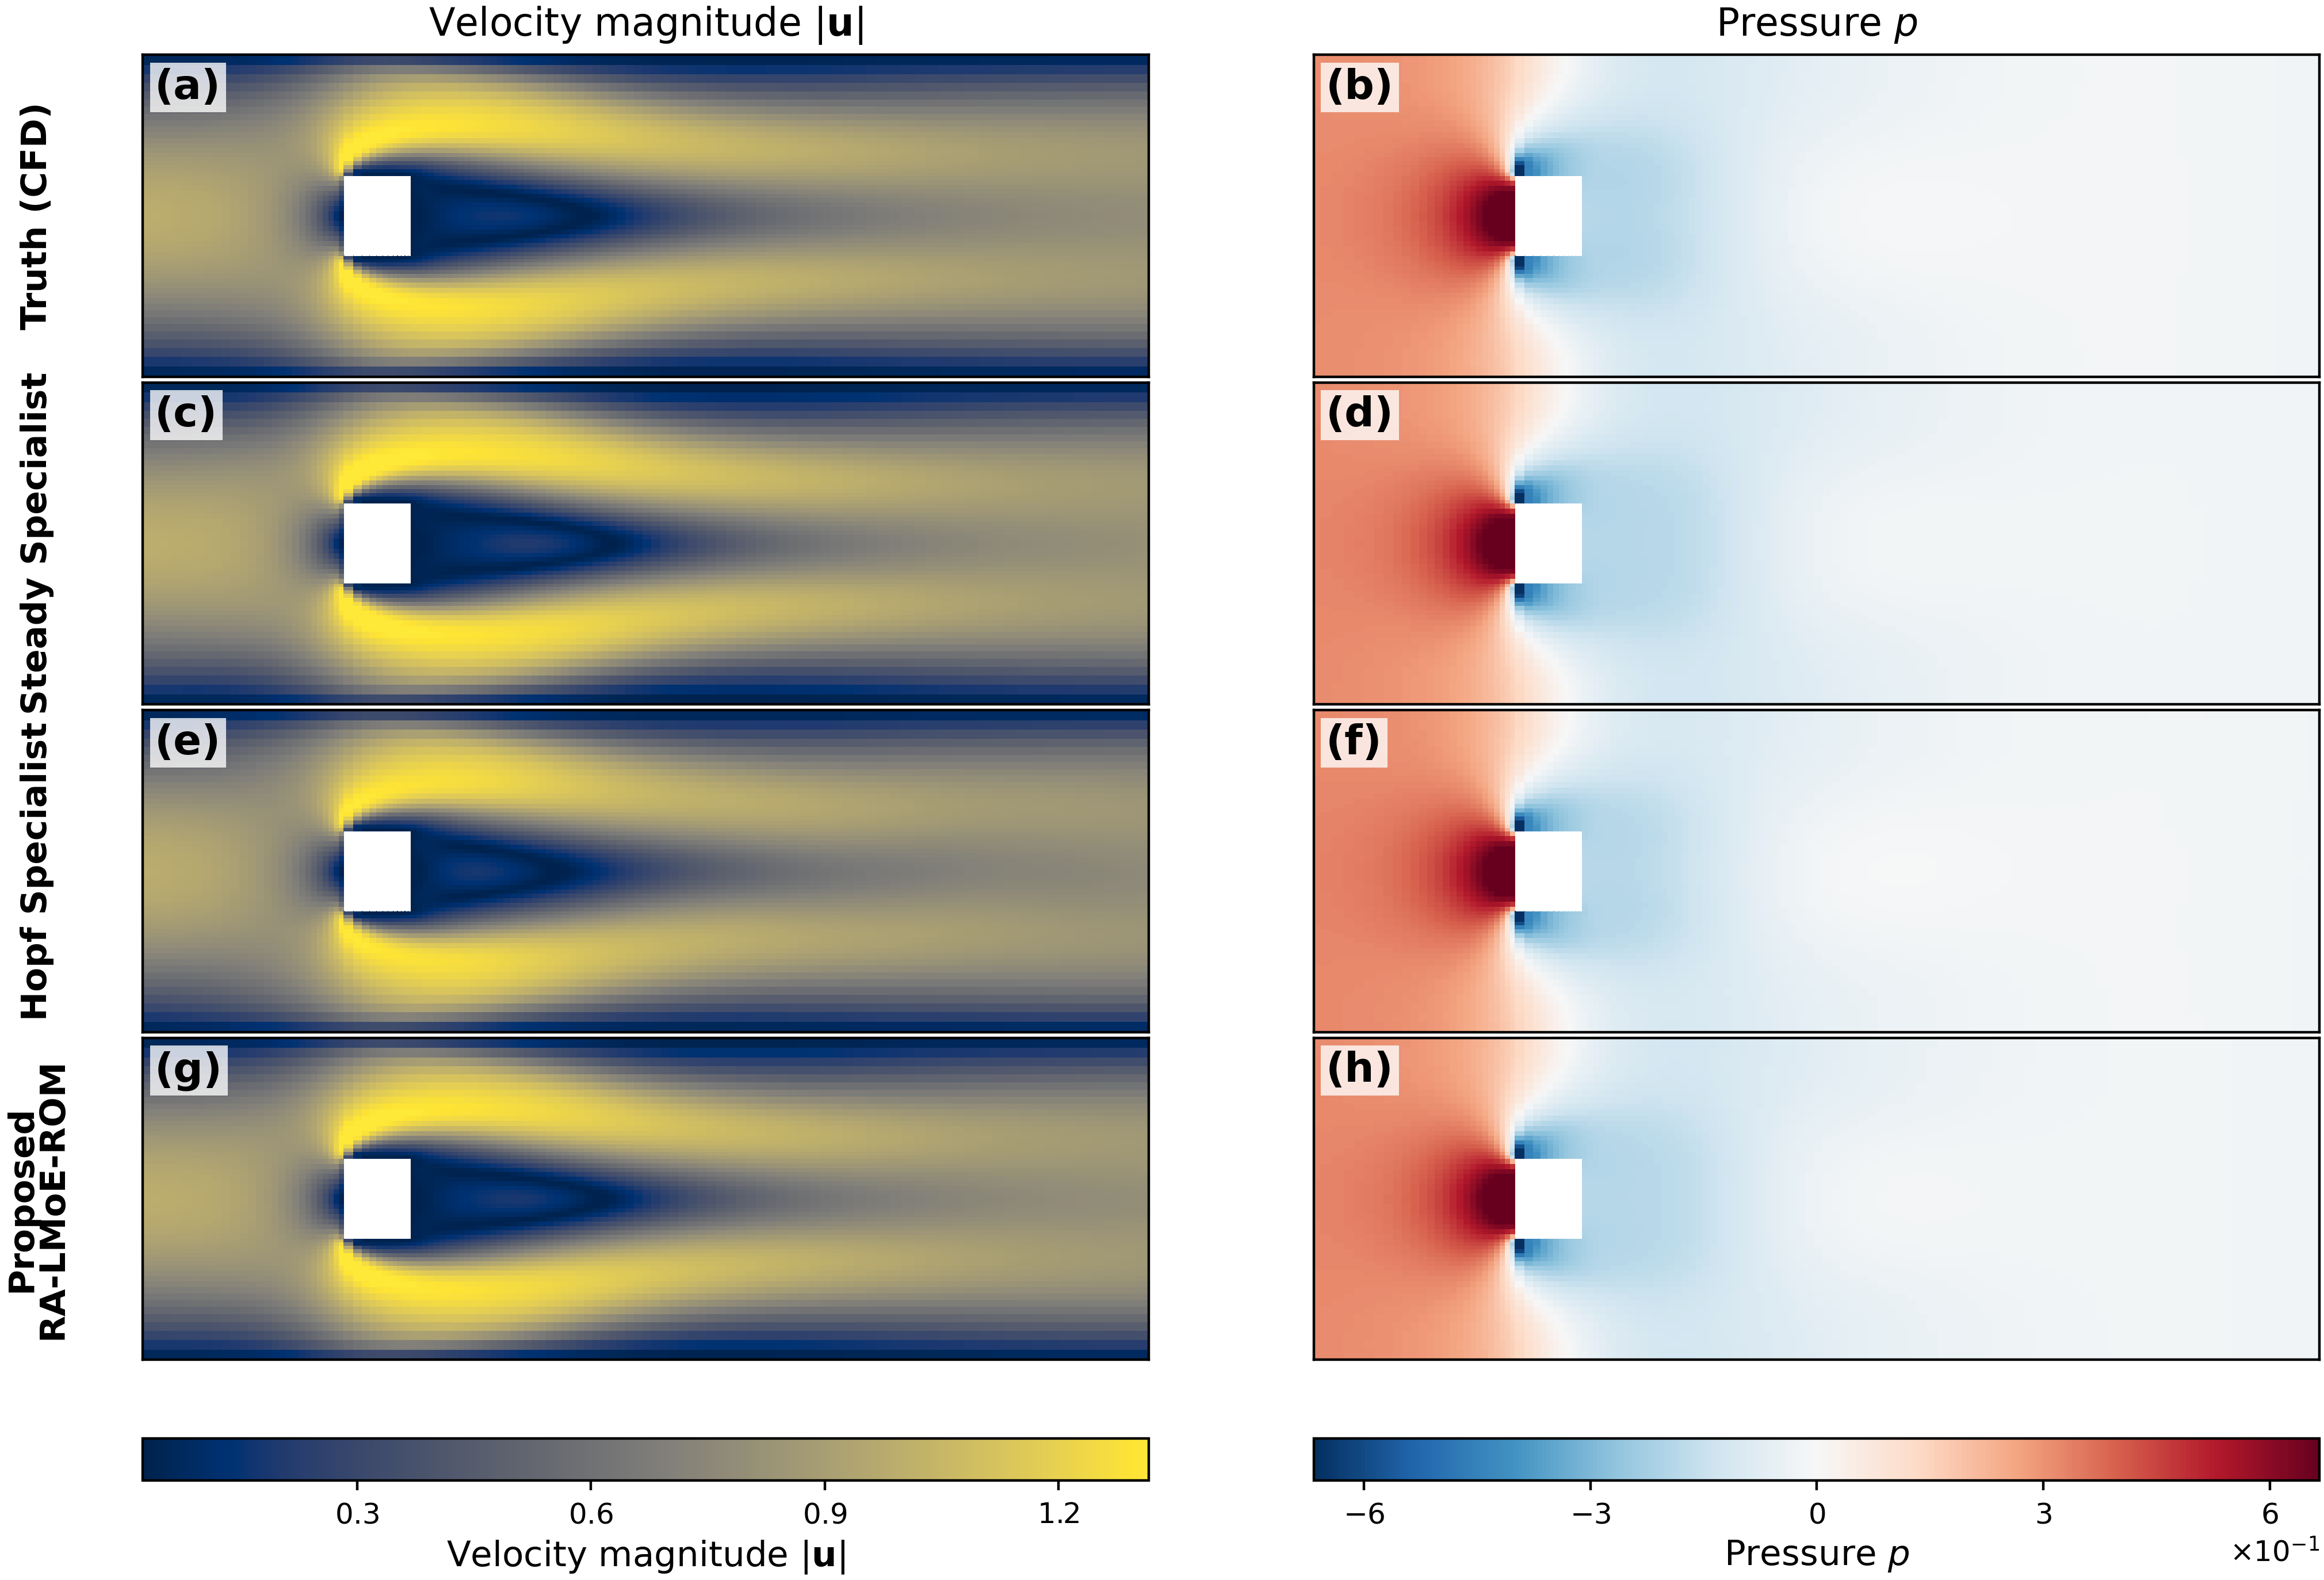
\includegraphics[width=0.80\linewidth]{figures/original/SH_2.png}

\vspace{0.35em}
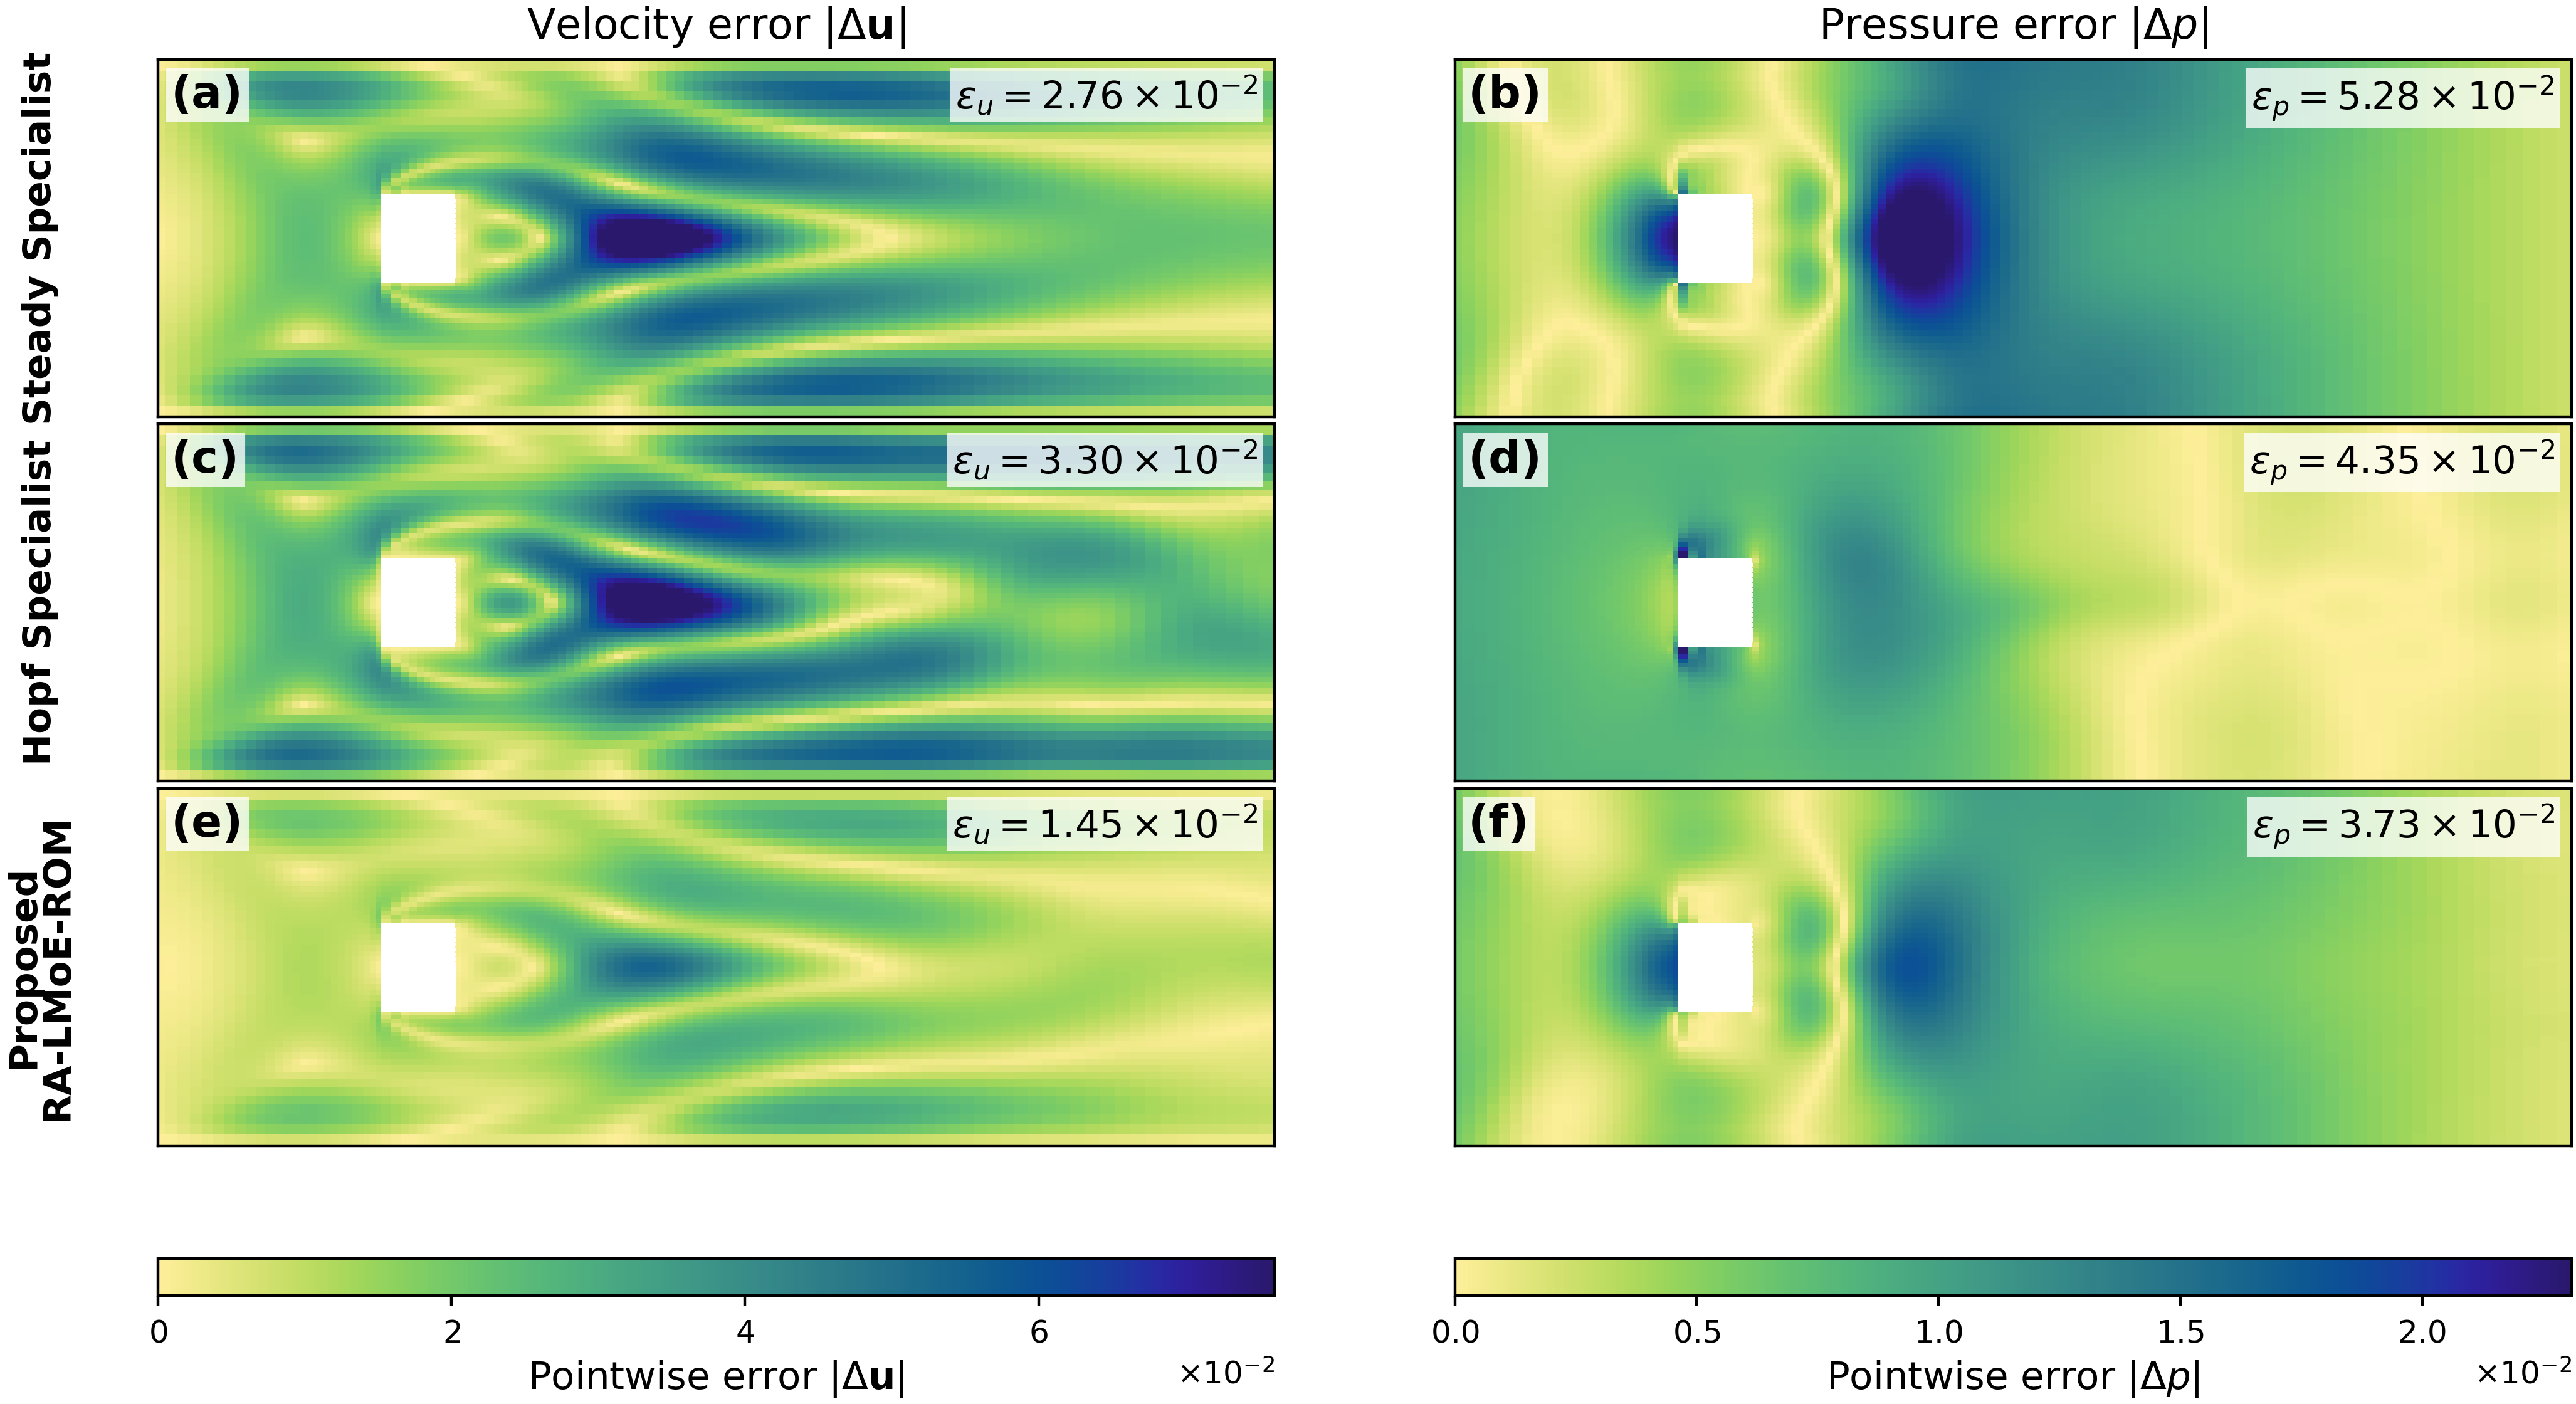
\includegraphics[width=0.80\linewidth]{figures/original/SH_2_1.png}
\caption{Representative held-out prediction in the centered-square
$S$--$H$ overlap at $Re=95.1$. The upper panel compares the CFD reference,
Steady specialist, Hopf specialist, and T2-C prediction for velocity
magnitude and gauge-corrected pressure. The lower panel gives the
corresponding pointwise absolute errors.}
\label{fig:app_square_sh_full}
\end{figure}
\par

\par
\begin{figure}[p]
\centering
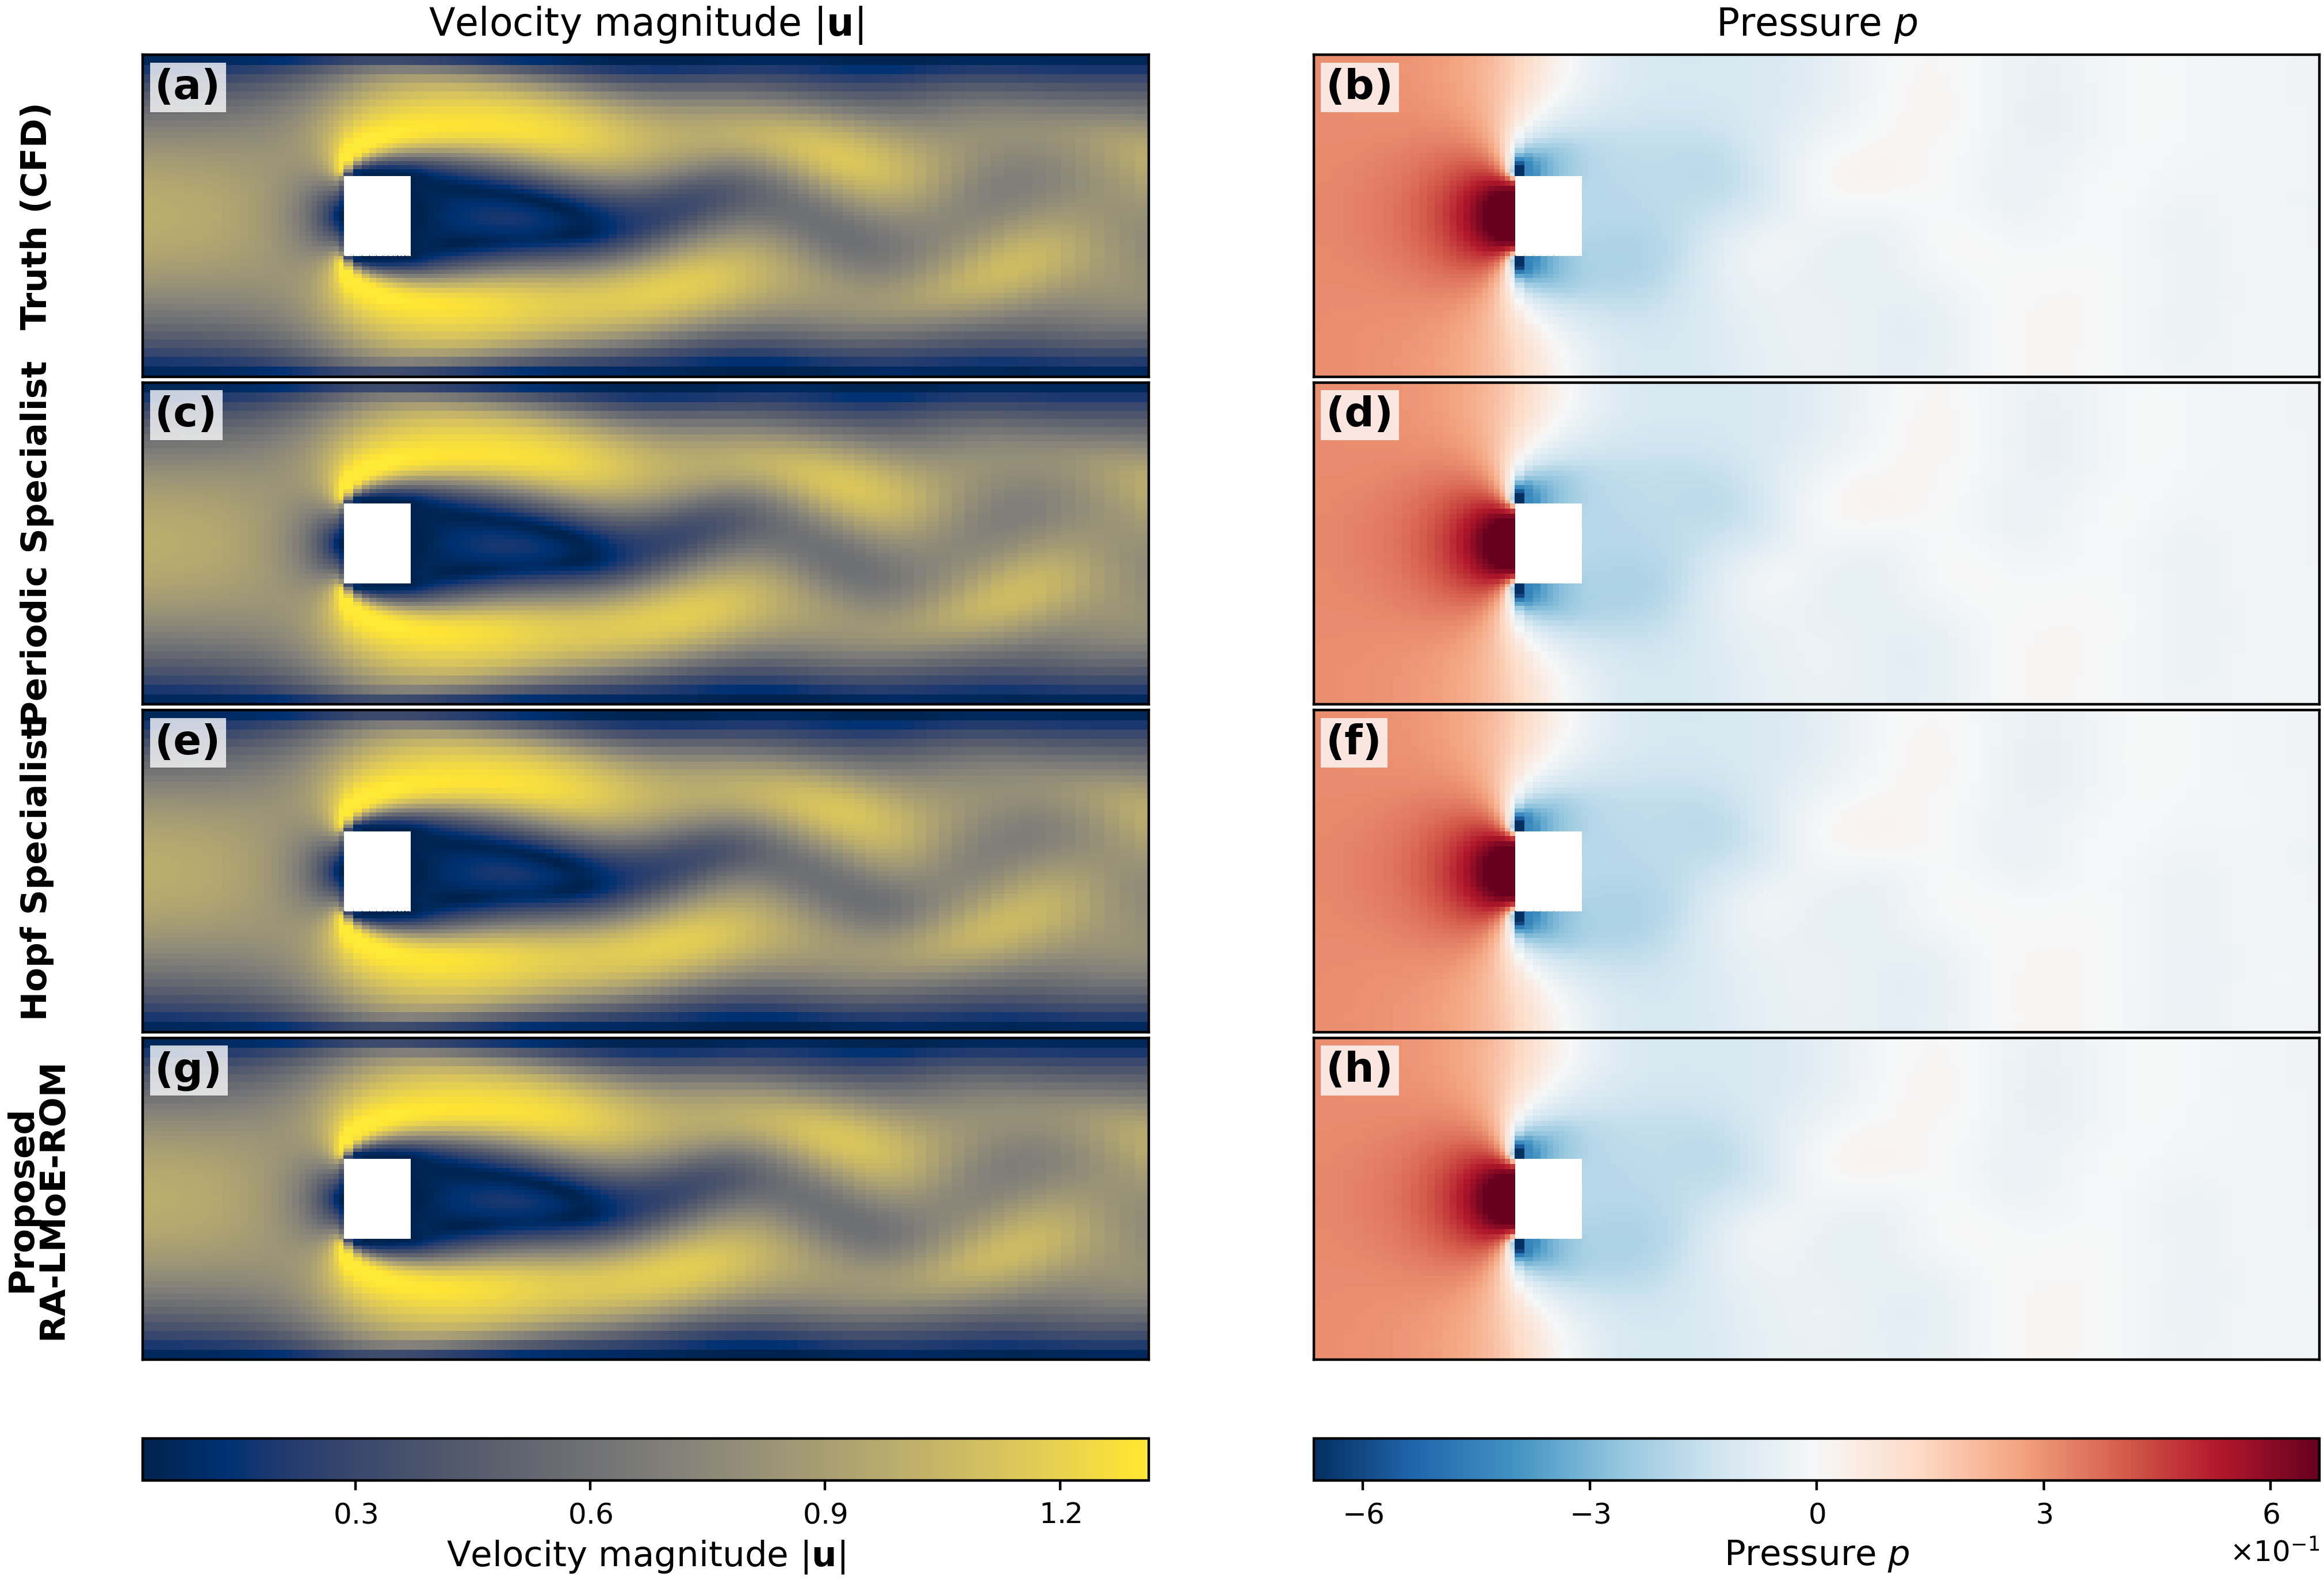
\includegraphics[width=0.80\linewidth]{figures/original/HP_2.png}

\vspace{0.35em}
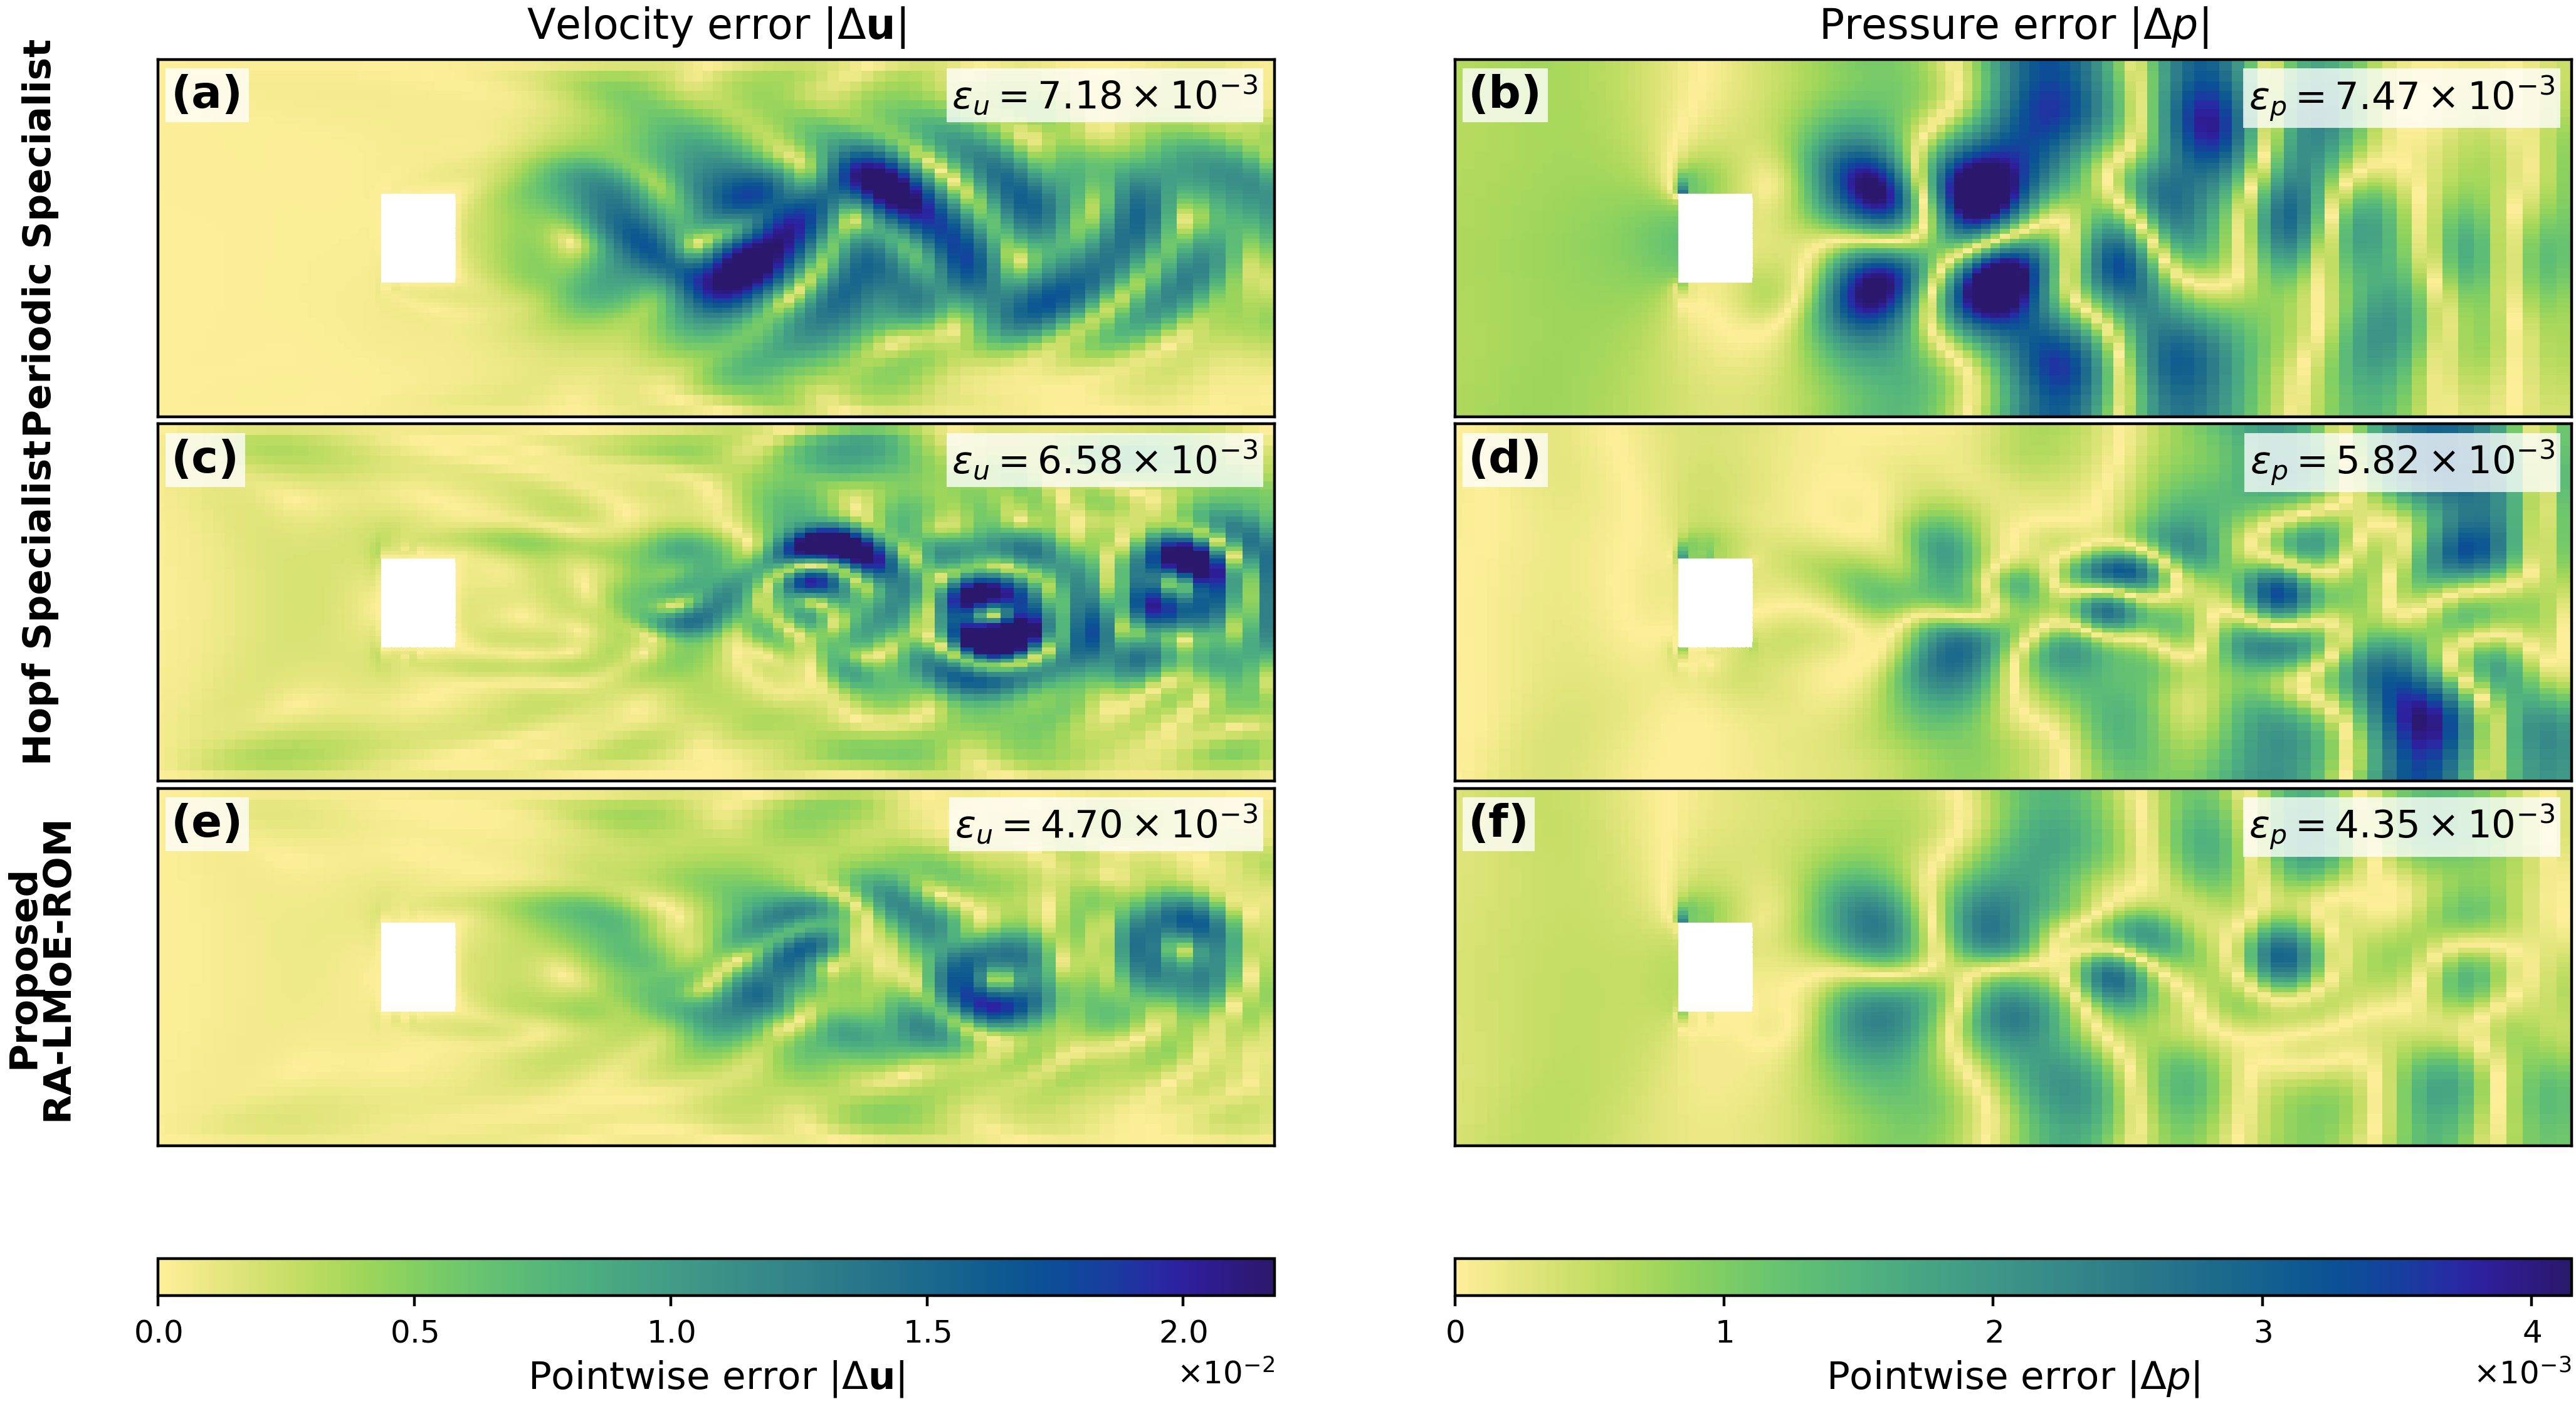
\includegraphics[width=0.80\linewidth]{figures/original/HP_2_1.png}
\caption{Representative held-out prediction in the centered-square
$H$--$P$ overlap at $Re=100.5$. The upper panel compares the CFD reference, Periodic specialist, Hopf specialist, and T2-C prediction for velocity magnitude and gauge-corrected pressure. The lower panel gives the
corresponding pointwise absolute errors.}
\label{fig:app_square_hp_full}
\end{figure}
\par

\FloatBarrier
\section{Fluidic-pinball results}
\label{app:pinball}

The POD--DeepONet baseline provides a complementary comparison between
one-step prediction and autonomous rollout. It attains $E_u=1.5921\%$ and $E_p=23.3447\%$ on 4,228 held-out input--output pairs, but only 1 of 28 held-out trajectories completes the prescribed autonomous rollout evaluation. This difference illustrates that one-step accuracy does not by itself imply reliable autonomous prediction. Because the POD--DeepONet evaluation uses a different temporal cadence from
the Periodic specialist, it is used only for this comparison of one-step prediction and autonomous rollout and not as a cadence-matched long-horizon accuracy baseline.

\paragraph{Periodic-core evaluation protocol.}
The $K=32$ Periodic result in Table~\ref{tab:pinball_autonomous} corresponds to the standard periodic evaluation. We additionally report a longer $K=56$ evaluation restricted to the Periodic-core final-test trajectories. The full-order snapshots are stored every $0.25$ physical time units; subsampling every fourth snapshot gives an effective interval $\Delta t=1$, matching the Periodic specialist's native history cadence. The $K=56$ setting therefore provides a longer autonomous evaluation within the same periodic regime without changing the specialist representation or
sampling convention.

\par
\begin{table}[H]
\centering
\caption{
Fluidic-pinball overlap joint errors (\%). For $S$--$H$, Candidate~1 is the Steady specialist and Candidate~2 is Hopf; for $H$--$P$, Candidate~1 is the Periodic specialist and Candidate~2 is Hopf.
The convex oracle selects its weight a posteriori for each evaluation window and is unavailable during prediction.
}
\label{tab:pinball_overlap}
\small
\setlength{\tabcolsep}{3.5pt}
\begin{tabular}{lrccccc}
\toprule
Overlap & $K$ & Cand.~1 & Cand.~2 & E2-probability blend & T2-C & Convex oracle \\
\midrule
$S$--$H$ & 24 & 0.6014 & 3.1925 & 1.7511 & 0.5897 & \textbf{0.5889} \\
$S$--$H$ & 56 & 0.6927 & 3.1193 & 1.7714 & 0.6767 & \textbf{0.6763} \\
$H$--$P$ & 24 & 0.0990 & 0.5146 & 0.2972 & 0.0945 & \textbf{0.0928} \\
$H$--$P$ & 56 & 0.1028 & 0.5346 & 0.3085 & 0.0978 & \textbf{0.0955} \\
\bottomrule
\end{tabular}
\end{table}
\par

T2-C improves upon Candidate~1 in all four overlap evaluations.
The relative reductions in joint error are approximately $1.9\%$ and
$2.3\%$ for $S$--$H$ at $K=24$ and $K=56$, and $4.5\%$ and $4.9\%$
for $H$--$P$, respectively. Although these gains are more modest than those observed for the centered-square benchmark, they persist at both rollout horizons. T2-C also remains close to the corresponding window-wise convex oracle, indicating that the learned fusion captures most of the available benefit from convex physical-space assembly in these overlap evaluations.

\FloatBarrier
\section{Additional internal-routing diagnostics}
\label{app:internal_routing}

\paragraph{Evaluation protocol and routing statistics.}
We analyze the frozen circular-cylinder Hopf and Periodic specialists on their held-out autonomous rollout windows.
For the Periodic specialist, we use 13 fixed windows at each of four held-out Reynolds numbers, giving 52 windows of length $K=48$. For the Hopf specialist, we use five fixed windows at each of three held-out Reynolds numbers, giving 15 windows of length $K=56$. One routing record is collected per reduced time step at the first integration stage, resulting in 2496 Periodic and 840 Hopf routing decisions per channel. Thus the reported statistics characterize reduced time step routing rather than all intermediate right-hand-side evaluations. Overlapping windows are not interpreted as independent trajectories, and these diagnostics are not used for model selection.

For $N$ routing decisions, let $I_{n,e}\in\{0,1\}$ indicate whether routed expert $e$ is selected at decision $n$, with the group identity included in the expert label. We define the normalized activation frequency
\begin{equation}
  f_e
  =
  \frac{1}{2N}
  \sum_{n=1}^{N} I_{n,e},
  \label{eq:app_routing_frequency}
\end{equation}
where the factor $2$ accounts for the Top-2 routed experts selected at each decision, so that $\sum_e f_e=1$. The corresponding mean routing mass is
\begin{equation}
  m_e
  =
  \frac{1}{N}
  \sum_{n=1}^{N}
  \omega_{n,e}I_{n,e},
  \label{eq:app_routing_mass}
\end{equation}
where $\omega_{n,e}$ denotes the final routed mixing coefficient assigned to expert $e$. Experts that are never selected are retained with $f_e=m_e=0$.

We summarize the dispersion of expert selection by the normalized utilization entropy
\begin{equation}
  H
  =
  -\frac{
    \sum_{e:f_e>0} f_e\log f_e
  }{
    \log N_E
  },
  \qquad
  0\le H\le1,
  \label{eq:app_routing_entropy}
\end{equation}
where $N_E$ is the number of routed experts available to the corresponding channel. Because $H$ is computed from activation frequency rather than routing mass, it characterizes diversity of expert selection rather than equality of the assigned weights. Distinct Top-2 pairs retain group identity but are treated as unordered.

For the two specialists considered here, the architecture assigns a fixed coefficient $4/7$ to the shared expert and a total coefficient $3/7$ to the routed Top-2 component. Consequently,
\begin{equation}
  \sum_e m_e=\frac{3}{7}.
\end{equation}
The routing mass therefore measures mixture allocation; it does not quantify the norm of an expert output or, by itself, establish a physical interpretation.
Labels such as \texttt{g0:e0} refer only to routed experts and should not be confused with the shared expert $e=0$ in
Eq.~(\plaineqref{eq:app_channel_sparse_moe}).

\par
\begin{table}[H]
\centering
\caption{
Post-hoc internal-routing statistics for the circular-cylinder Hopf and Periodic specialists on held-out autonomous rollout windows. ``Dominant-pair share'' denotes the fraction of routing decisions associated with the most frequently selected unordered Top-2 pair. $H$ denotes the normalized utilization entropy defined in Eq.~(\plaineqref{eq:app_routing_entropy}).
}
\label{tab:internal_routing_summary}
\small
\setlength{\tabcolsep}{5pt}
\begin{tabular}{@{}llrrrr@{}}
\toprule
Specialist & Channel & \shortstack{Active\\experts} & \shortstack{Distinct\\Top-2 pairs} & \shortstack{Dominant-pair\\share (\%)} & $H$ \\
\midrule
Hopf & Velocity & 2/6 & 1 & 100.00 & 0.387 \\
     & Pressure & 2/6 & 1 & 100.00 & 0.387 \\
\addlinespace
Periodic & Velocity & 18/18 & 33 & 16.27 & 0.929 \\
         & Pressure & 14/18 & 16 & 31.25 & 0.784 \\
\bottomrule
\end{tabular}
\end{table}
\par

\paragraph{Periodic routing profile.}
The Periodic specialist uses a broad range of its available routed experts. Across the held-out rollouts, the velocity channel selects all 18 routed experts and realizes 33 distinct group--pair combinations, while the pressure channel selects 14 of 18 experts through 16 combinations (Table~\ref{tab:internal_routing_summary}). The most frequent pair accounts for only $16.27\%$ of velocity decisions and $31.25\%$ of pressure decisions, consistent with the higher utilization entropy of the velocity channel. The selected groups also vary across the four held-out Reynolds numbers.
Figure~\ref{fig:periodic_internal_routing} summarizes the corresponding group frequencies and routed-expert masses.



\paragraph{Hopf routing profile.}
The Hopf specialist exhibits a substantially more concentrated routing pattern. Because it contains a single expert group, only channel-level routing is active. Across all evaluated windows, the velocity channel selects the pair
$(e_1,e_3)$ and the pressure channel selects $(e_2,e_4)$ at every recorded reduced time step. A separate stage-wise check confirms that these same pairs are retained across all four Runge--Kutta stages.

Although the selected support is fixed, the routed weights are strongly nonuniform. Velocity expert $e_3$ receives approximately $99.93\%$ of the total routed mass, while pressure expert $e_2$ receives $84.16\%$. The secondary pressure expert $e_4$ nevertheless receives a Reynolds-number-dependent weight, with its mean mass increasing across the three held-out parameter values.

The two specialists therefore exhibit different internal utilization patterns. The Periodic specialist distributes routing decisions across many group--pair combinations, whereas the Hopf specialist retains fixed sparse support and adapts primarily through the mixture weights. The single Hopf group is part of the prescribed architecture and should not be interpreted as collapse of a learned multi-group router.

\paragraph{Periodic rollout-position diagnostic.}
Figure~\ref{fig:periodic_routing_step} shows the mean routed-expert mass as a function of normalized rollout position, using the same 52 held-out Periodic windows. The horizontal coordinate reflects prediction position within the
autonomous window rather than physical oscillation phase. This diagnostic complements the aggregate statistics above by showing how expert allocation varies over the autonomous rollout.


\par
\begin{figure}[H]
\centering
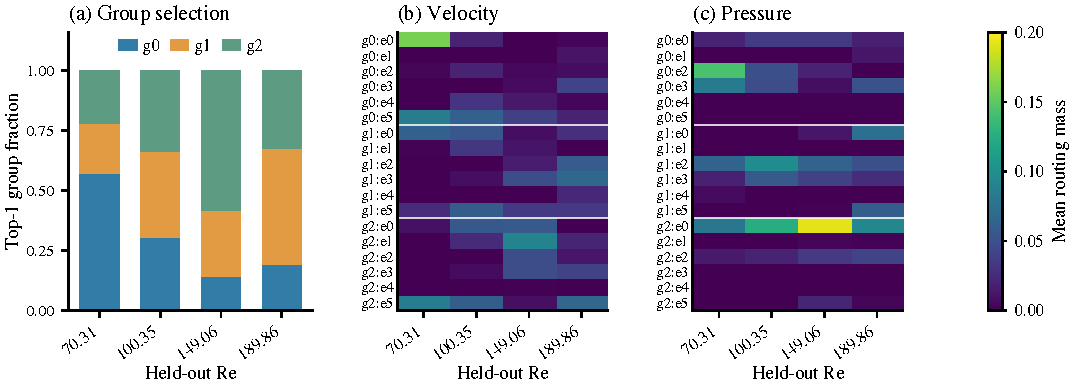
\includegraphics[width=\linewidth]{figures/periodic_internal_routing.pdf}
\caption{
Internal routing of the circular-cylinder Periodic specialist on held-out autonomous rollouts, recorded once per reduced time step at the first integration stage. (a) Top-1 group-selection frequencies. (b,c) Mean routed-expert mass for the velocity and pressure channels. Expert identifiers are local to the corresponding specialist, group, and channel and are not assigned physical labels.
}
\label{fig:periodic_internal_routing}
\end{figure}
\par

\par
\begin{figure}[H]
\centering
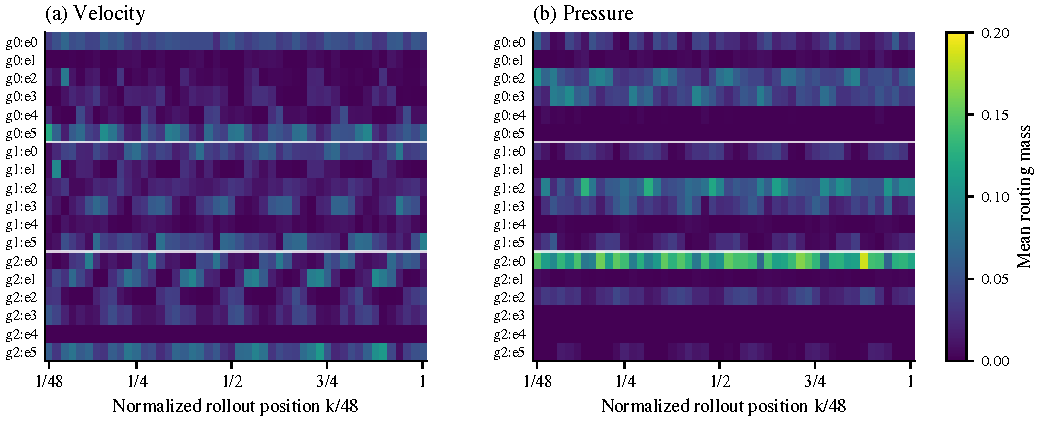
\includegraphics[width=\linewidth]{figures/periodic_rollout_step_routing.pdf}
\caption{
Routed-expert mass versus autonomous rollout position for the circular-cylinder Periodic specialist. Each column averages the routing decision at the corresponding reduced time step over the 52 fixed held-out windows, and all routed experts are retained. The horizontal coordinate is the normalized prediction position $k/48$ and is not interpreted as physical oscillation phase.
}
\label{fig:periodic_routing_step}
\end{figure}
\par

\clearpage
\section{Trainable and active parameter counts}
\label{app:parameter_counts}

\paragraph{Counting convention.}
Total parameters count unique trainable parameters in each analyzed
circular-cylinder specialist. Active parameters count unique trainable
parameters used by one batch-size-one prediction-path routing decision,
not their union across a batch, trajectory, or all RK4 stages. These include
the encoder and refinement blocks, executed routers, the selected group's
shared experts, channel-specific Top-2 velocity and pressure experts, and
the learned pressure correction. Fixed POD bases, projected operators,
normalization statistics, and non-trainable buffers are excluded.

\par
\begin{table}[H]
\centering
\caption{Trainable and per-decision active parameter counts for the analyzed
circular-cylinder specialists. Active counts refer to the sparse prediction
path; M denotes one million parameters.}
\label{tab:parameter_counts}
\begin{tabular}{lrrr}
\toprule
Specialist & Total trainable & Active prediction & Active fraction \\
\midrule
Hopf & 31.81M & 14.17M & 44.53\% \\
Periodic & 48.62M & 8.31M & 17.09\% \\
\bottomrule
\end{tabular}
\end{table}
\par

The Hopf and Periodic specialists activate 44.53\% and 17.09\% of their
trainable parameters per prediction decision, respectively. These counts
describe conditional parameter activation, not measured FLOPs, runtime,
or speedup. Complete parameter-matched counts are unavailable for the
Vanilla-FNN-MoE, DataOnly-MoE, and Global MoE ablations, so the local
architecture comparison is not interpreted as a capacity-matched study.


\end{document}
